\documentclass[12pt,bibliography=totocnumbered,listof=totocnumbered,abstracton]{scrreprt}
\usepackage[paper=a4paper,left=30mm,right=30mm,top=30mm,bottom=30mm]{geometry}
\usepackage[utf8]{inputenc}
\usepackage[hyphens]{url}
%\usepackage{pdfcomment}
\usepackage[ngerman]{babel}
\usepackage{tocstyle}
\usetocstyle{allwithdot}
\usepackage{lmodern}
\usepackage[numbers, sort&compress]{natbib}
\usepackage{graphicx} 
\usepackage{subfigure} 
\usepackage{filecontents}
\usepackage[T1]{fontenc}
\usepackage{pifont}
\usepackage{setspace}
\usepackage{amsmath}
\usepackage[automark]{scrpage2}

\begin{filecontents}{books.bib}

@MISC{winrichtlinien,
author = "{Microsoft Corporation}",
year = "2014",
title = "Windows App Development: Guidelines for targeting",
howpublished = "\url{http://msdn.microsoft.com/en-us/library/windows/apps/hh465326.aspx}",
note = "Zuletzt aufgerufen am 06.08.2014"
}

@MISC{applerichtlinien,
author = "{Apple Inc.}",
year = "2014",
title = "iOS Human Interface Guidelines: Layout",
howpublished = "\url{https://developer.apple.com/library/ios/documentation/UserExperience/Conceptual/MobileHIG/LayoutandAppearance.html}",
note = "Zuletzt aufgerufen am 09.08.2014"
}

@MISC{androidrichtlinien,
author = "{Open Handset Alliance™}",
year = "2014",
title = "Android Developers: Metrics and Grids",
howpublished = "\url{http://developer.android.com/design/style/metrics-grids.html}",
note = "Zuletzt aufgerufen am 09.08.2014"
}

@MISC{sonyverge,
author = "Dante D'Orazio",
year = "2012",
title = "Sony Xperia Sola's 'floating touch' screen technology explained",
howpublished = "\url{http://www.theverge.com/2012/3/14/2871193/sony-xperia-sola-floating-touch-hover-event-screen-technology}",
note = "Zuletzt aufgerufen am 07.08.2014"
}

@ARTICLE{monkeys,
author = "K. Dandekar, B.I. Raju, M.A. Srinivasan",
title = "3-D finite-element models of human and monkey fingertips to investigate the mechanics of tactile sense",
pages = "S. 682-691",
year = "2003",
journal = "Journal of biomechanical Engineering",
volume = "125"
}

@INCOLLECTION{jin,
author = "Zhao Xia Jin, Tom Plocher, Liana Kiff",
title = "Touch screen user interfaces for older adults: button size and spacing",
booktitle = "Proceedings of the 4th international conference on Universal access in human computer interaction: coping with diversity (UAHCI'07)",
publisher = "Springer Verlag",
year = "2007",
editor = "Constantine Stephanidis",
pages = "933-941",
address = "Berlin, Heidelberg"
}

@ARTICLE{touchmouse,
author = "Charlotte Travis, Pietro Murano",
title = "A comparative study of the usability of touch-based and mouse-based interaction",
journal = "Int. J. Pervasive Computing and Communications",
volume = "10",
number = "1",
year = "2014",
pages = "115-134"
}

@MISC{dorol,
author = "{Doro Deutschland}",
year = "2014",
title = "Doro Liberto 810",
howpublished = "\url{http://www.dorodeutschland.de/Produkte/Mobiltelefone-und-Zubehor/Doro-Liberto-810/}",
note = "Zuletzt aufgerufen am 24.08.2014"
}

@MISC{gOne,
author = "Andreas Brohme",
year = "2014",
title = "Android One: Google startet seine Billig-Smartphone-Offensive",
howpublished = "\url{http://www.spiegel.de/netzwelt/gadgets/android-one-google-soll-billig-smartphone-bald-praesentieren-a-989376.html}",
note = "Zuletzt aufgerufen am 04.09.2014"
}

@INPROCEEDINGS{mousetouchmk,
author = "Farzan Sasangohar, I. Scott MacKenzie, Stacey D. Scott",
title = "Evaluation of mouse and touch input for a tabletop display using Fitts' reciprocal tapping task",
booktitle = "Proceedings of the Human Factors and Ergonomics Society Annual Meeting",
volume = "53",
number = "12",
pages = "839-843",
year = "2009", 
organization = "SAGE Publications"
}

@MISC{synaptics,
author = "{Synaptics Inc.}",
year = "1998",
title = "Synaptics TouchPad Interfacing Guide (510-000080-A, Second Edition)",
howpublished = "\url{http://www.synaptics.com/sites/default/files/ACF126.pdf}",
note = "Zuletzt aufgerufen am 18.08.2014"
}

@BOOK{nui,
author = "Daniel Wigdor, Dennis Wixon},
title = "Brave NUI World: Designing Natural User Interfaces for Touch and Gesture",
year = "2011",
edition = "1st",
publisher = "Morgan Kaufmann Publishers Inc.",
address = "San Francisco, CA, USA",
}

@INCOLLECTION{sus,
address = "London",
author = "Brooke, John",
booktitle = "Usability evaluation in industry",
editor = "Jordan, P. W. and Weerdmeester, B. and Thomas, A. and Mclelland, I. L.",
publisher = "Taylor and Francis",
title = "SUS: A quick and dirty usability scale",
year = "1996"
}

@ARTICLE{sus2013,
title = "SUS: A Retrospective",
author = "Brooke, John",
journal = "Journal of Usability Studies",
volume="8",
number="2",
pages="29-40",
year="2013"
}


@ARTICLE{fitts,
author = "I. Scott MacKenzie",
title = "Fitts' Law As a Research and Design Tool in Human-computer Interaction",
journal = "Hum.-Comput. Interact.",
issue_date = "March 1992",
volume = "7",
number = "1",
year = "1992",
pages = "91-139",
numpages = "49",
publisher = "L. Erlbaum Associates Inc.",
address = "Hillsdale, NJ, USA",
} 
\end{filecontents}

% Stil der Seiten
\pagestyle{scrheadings}
\clearscrheadfoot

%Abstand eines neuen Absatzes
\setlength{\parskip}{1em}
\setlength{\parindent}{0em}

%Abstand der Fussnoten
\deffootnote{1em}{1em}{\textsuperscript{\thefootnotemark\ }}

%Zeilenabstand
\onehalfspacing

%Regeln, bis zu welcher Tiefe Überschriften angezeigt werden sollen (Anzeige der berschriften im Verzeichnis / Anzeige der Nummerierung)
\setcounter{tocdepth}{3}
\setcounter{secnumdepth}{3}

%Kopfzeile
\ohead{\textbf{\headmark}\rlap{\hspace{1.5em}\rule[-0.7ex]{2pt}{\baselineskip}\hspace{1.5em}\thechapter}}

%Fußzeile
\ofoot{\rlap{\hspace{1.5em}\rule[-0.7ex]{1pt}{\baselineskip}\hspace{1.5em}\pagemark}}

%Kopf- und Fußzeile auch auf chapter-Seiten.
\renewcommand*{\chaptermarkformat}{}

%Schriftarten
\addtokomafont{pagenumber}{\sffamily \upshape}
\addtokomafont{pageheadfoot}{\sffamily \upshape}

%-------------------
%Ende des Kopfbereiches
%-------------------

%START---------------------------------------------------------------------------------
\begin{document}
\pagestyle{empty}
\pagenumbering{roman}
%Beginn der Titelseite
\begin{titlepage}
\begin{center}
\null
\vfill
\LARGE\textsf{\textbf{Unterstützung der Touchinteraktion durch Annäherungserkennung auf Smartphones.}}

\vfill
\LARGE\textrm{\textbf{Bachelorarbeit}}

\large\textrm{Fachbereich Mathematik und Informatik\\
\vspace{.5em}
Universität Bremen}

\vfill
\large\textsc{Zur Erlangung des akademischen Grades}\\
\vspace{.75em}
\textbf{Bachelor of Science (B.Sc.)}\\
\vspace{.75em}
\textsc{in Digitale Medien.}

\vfill\small\textsc{
Vorgelegt von\\
Jan-Hendrik Wolf\\
Geboren am 19. März 1991\\
Matrikel-Nr: 2616233}\\
%Mainstraße 36\\
%28199 Bremen\\
%\ding{38} 0151 15530761\\
%\ding{41} mail@jan-wolf.de\\
\vspace{1cm}
\small\textbf{Erstgutachter:  Prof. Dr. Rainer Malaka\\
Zweitgutachter: Dr.-Ing. Dennis Krannich}\\
\vspace{1cm}
\small\textsc{Bremen, 30. September 2014}
%Sommersemester 2014
\end{center}
\end{titlepage}
%Ende der Titelseite

%Inhaltsverzeichnis (aktualisiert sich erst nach dem zweiten Setzen)
\tableofcontents
%Beginn einer neuen Seite

%START-----------------------------------------------------------------------------------
\chapter*{Danksagung}
Hiermit möchte ich mich bei allen Personen herzlich bedanken, die mich während der Anfertigung dieser Bachelorarbeit unterstützt haben.

Besonders bedanken möchte ich mich bei\dots
\begin{itemize}
\item Frederic Pollmann für die außerordentliche Betreuung und den vielen von ihm beantworteten E-Mails.
\item Nina Runge für die hilfreichen Tipps.
\item Prof. Dr. Rainer Malaka und Dr.-Ing. Dennis Krannich für die Einwilligung als Erst- und Zweitprüfer.
\item allen Testteilnehmern meiner Studie für die freiwillige Unterstützung.
\item meinen Korrekturlesern X, X, X.
\item meiner Familie für die tolle Unterstützung und Hilfe neben und während dieser Arbeit.
\end{itemize}

\chapter*{Zusammenfassung}
Für ein verbessertes Verständnis der Usability von Annäherungserkennung und zur Überprüfung der Mindestgrößen von Bedienelementen wurde im Rahmen dieser Bachelorarbeit eine Studie durchgeführt. Insgesamt durchliefen 18 Testpersonen verschiedene Aufgaben innerhalb einer Testanwendung. Durch mehrmalige Wiederholungen der Aufgaben unter Veränderung der jeweiligen Zustände der Annäherungserkennung wurde anhand der erhobenen Daten die Unterschiede mehrerer Parameter bestimmt.

Es konnte gezeigt werden, dass die Annäherungserkennung für die Aufgabenerledigung nach Meinung der Nutzer unterstützend wirkte. Für die üblichen Schaltflächengrößen unterschied sich die Anzahl der verblieben Testpersonen im Test jedoch kaum. Bei aktivierter Annäherungserkennung bzw. bei aktivierter Selektionshilfe konnten lediglich bei Schaltflächengrößen zwischen $2.4$ mm  und $1.4$ mm signifikant mehr Testpersonen im Test verbleiben. Weiterhin wurden für jede Testperson die Parameter nach Fitt's Law ermittelt. Dabei erhöhte sich mit eingeschalteter Annäherungserkennung die Zeitdauer bis zur endgültigen Ausführung einer Interaktion. Bei ausgeschalteter Annäherungserkennung war die Zeitdauer am geringsten und während der aktivierten Selektionshilfe am größten. Die Unterschiede jeder Zeitdauer waren bei allen Kombinationen signifikant unterschiedlich.

\pagenumbering{arabic}
\pagestyle{scrheadings}
\chapter{Einleitung}
Im Alltag wird die Entwicklung des "`Ubiquitous computing"' für viele Anwender zunehmend sichtbar. Viele periphere Geräte, wie z.B. in Bereichen der Haussteuerung, Überwachungstechnik und dem Unterhaltungsbereich beinhalten mittlerweile Computerchips, die sich über Smartphones vieler unterschiedlicher Hersteller konfigurieren und steuern lassen. Das Smartphone ist somit als Steuerungszentrale im "`Internet der Dinge"' ein wichtiger Bestandteil geworden.\\
Somit ist es nicht verwunderlich, dass stetig neue Geräte dieser Art für unterschiedlichste Zielgruppen auf den Markt gebracht werden. Mittlerweile bieten sogar etablierte Hersteller bekannter Seniorenhandys Varianten in Form von Smartphones an \citep{dorol}. Mit Einsteigergeräten, wie z.B. dem "`Google One"' \citep{gOne}, werden auch Menschen mit geringem Einkommen angesprochen. Durch diese stetige Verbreitung nimmt gleichzeitig die Wichtigkeit einer adäquaten Interaktion auf mobilen Endgeräten zu.

Aufgrund der Tatsache, dass Anwender von den bisher weit verbreiteten Desktop-PCs und Laptops an große Bedienoberflächen mit umfangreichen Funktionen gewöhnt sind, besteht die Herausforderung auf mobilen Endgeräten auch darin, Anwendungen auf kleineren Bildschirmen ähnlich funktional auszustatten. Dies erfordert eine effiziente Ausnutzung der verfügbaren Bildschirmfläche.\\
Im Bezug auf die Eingabe zählt bei Desktop-PCs und Laptops die Maus und Tastatur zu den etablierten Eingabegeräten.  Mobile Endgeräte sind jedoch nur dann besonders sinnvoll, wenn keine zusätzlichen Eingabegeräte nötig sind. Damit das Mitführen eines zusätzlichen Eingabegerätes entfällt, erfolgt die Interaktion auf vielen mobilen Endgeräten hauptsächlich über die Fingerberührung unter Mitnutzung zusätzlicher Sensoren, wie z.B. Neigungs- und Lichtsensoren. Zudem stellt sich der Finger als intuitives Eingabegerät heraus und erleichtert damit das Anwählen von Schaltflächen auf dem Bildschirm. Ab einer bestimmten Schaltflächengröße erhöht sich jedoch die Fehlerrate der Interaktion \citep{mousetouchmk}.\\
Grund hierfür ist der fehlende Mauszeiger als indirektes Eingabegerät. Während die Position des Mauszeigers die Position der Interaktion definiert, weicht die Position des Fingers von der Position der Interaktion meist leicht ab, da der Finger eine größere Berührungsfläche besitzt. Zusätzlich verdeckt der Finger durch dessen Größe kleine Schaltflächen, wohingegen der Mauszeiger weiterhin eine präzise Selektion ermöglicht. Um diesem sogenannten "`Fat-Finger-Problem"' \citep{monkeys} entgegenzuwirken, ist die Mindestgröße der Bedienelemente auf diesen Bildschirmen im Vergleich zu Bedienelementen für Mausinteraktionen auf vielen Systemen vergrößert worden \citep{jin}.\\
Ein weiterer Vorteil der Mausinteraktion gegenüber der Interaktion durch Berührung ist der Umstand, dass die aktuelle Position des Mauszeigers auch vor dem Klicken auf der Bedienoberfläche sichtbar ist. Die Positionierung und der Klick mittels des Mauszeigers kann somit unabhängig voneinander erfolgen. Dies ermöglicht das Schweben des Mauszeigers über einer Schaltfläche und wird als "`Hovering"' (engl. "`Schweben"') bezeichnet. Auf Laptops und Desktop-PCs ist dies eine gängige Interaktionsform und wird meist verwendet, um die Eigenschaften von Objekten auf dem Bildschirm, wie z.B. das Aussehen, zu verändern. Durch derartige Eigenschaftsänderungen kann der Anwender das Objekt beispielsweise als Schaltfläche identifizieren.
\begin{figure}
\centering
\subfigure[Zusätzliche, visuelle Ebene: Bildschirmlupe]{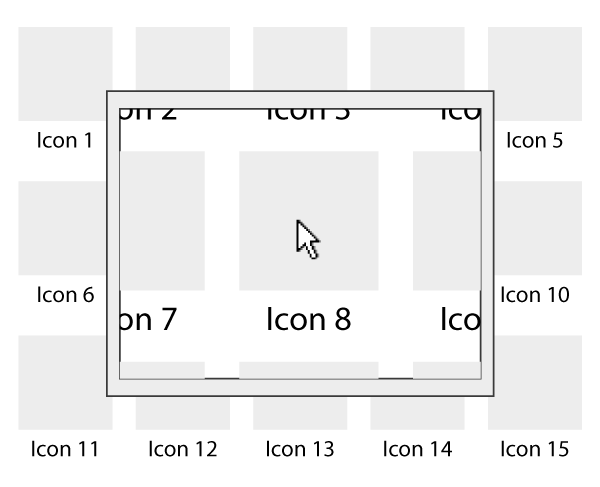
\includegraphics[width=0.49\textwidth]{img/einleitung1_hoverlupe.png}}
\hfill
\subfigure[Selektion ohne Ausführung: Menüauswahl]{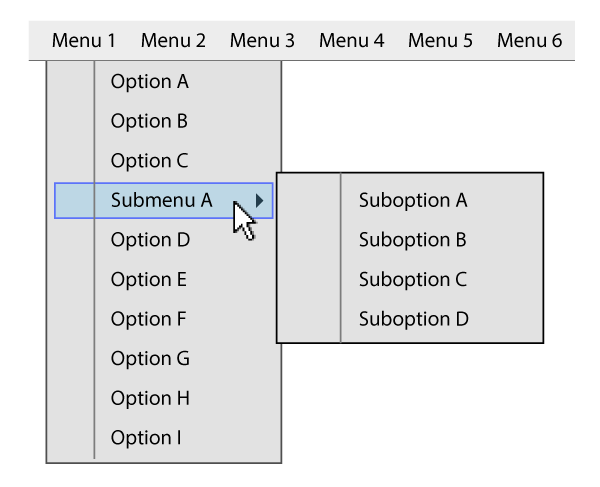
\includegraphics[width=0.49\textwidth]{img/einleitung1_hovermenu.png}}
\caption{Schematische Darstellung für "`Hovering"' als Interaktionsform.}
\label{hoveringdesktop}
\end{figure}
Abbildung \ref{hoveringdesktop} zeigt zwei Anwendungsbeispiele, die diese Interaktionsform nutzen.

Bisher war es jedoch nicht möglich, dass sogenannte "`Hovering"' in das Repertoire der Interaktionsformen mobiler Endgeräte zu übernehmen. Dies änderte sich nachdem Sony im Mai 2012 erstmals ein Smartphone mit integrierter Annäherungserkennung für den gesamten Markt veröffentlichte. In einigen nativen Anwendungen von Sony ließ sich nun auch diese Interaktionsform auf einem berührungsempfindlichen Bildschirm verwenden \citep{sonyverge}. Die Verbreitung und Integration der Annäherungserkennung ist bisher jedoch lediglich in einem kleinen Teil der Geräte erfolgt.

In der vorliegenden Bachelorarbeit soll untersucht werden, ob visuelle Hover-""Effekte auf berührungsempfindlichen Endgeräten mit integrierter Annährungserkennung die Usability von Bedienelementen im Bezug auf Geschwindigkeit und Präzision verbessern können und auf diese Weise eine beschleunigte Integration dieser Technologie gerechtfertigt werden kann. Um die visuelle Darstellung der Bedienoberfläche nicht essentiell zu verändern oder zu überlagern, werden die Untersuchungen insofern konkretisiert, sodass auf zusätzliche, visuelle Ebenen verzichtet wird.

\section{Gegenwärtiger Stand der Technik mobiler Endgeräte}
Zum jetzigen Zeitpunkt ist die Anzahl der mobilen Geräte mit integrierter Annäherungserkennung stark begrenzt. Zudem nutzen die Benutzungsoberflächen auf heutigen Smartphones mit Annäherungserkennung die Möglichkeiten der Technologie nur in vereinzelten Fällen aus. Im Folgenden soll ein kurzer Überblick auf die gegenwärtige Hardware und Software gegeben werden, die diese Annäherungserkennung unterstützt.

\subsection{Hardware}
Bereits im Jahr 1998 erwähnte der Touchpad-Hersteller Synaptics in einem Dokument die allgemeine Funktionsweise und diverse Spezifikationen zur Annäherungserkennung auf berührungsempfindliche Oberflächen und bestätigte damit die technische Möglichkeit \citep{synaptics}. Die Erkennung funktioniert theoretisch auf allen kapazitiven Oberflächen. Dazu wird die Kapazitätsstärke des jeweiligen Fingers ermittelt und anschließend die ungefähre Entfernung des Fingers zur Oberfläche approximiert.

Die Technologie erlangte jedoch erst im Jahr 2012 die Aufmerksamkeit der Öffentlichkeit. Sony vermarktete zu dieser Zeit mit dem Xperia™ sola das erste Smartphone mit Annäherungserkennung und bewarb die Technologie unter dem Namen Floating Touch™.\\
Zu Beginn des Jahres 2013 brachte als zweiter Hersteller auch Samsung mit dem Galaxy S4 ein Gerät mit ähnlicher Technologie namens AirView™ auf den Markt. Im Gegensatz zu Sony, integrierte Samsung im Jahr 2014 die Annäherungserkennung auch in das Nachfolgemodell, dem Samsung Galaxy S5.

\subsection{Software}
In mobilen Endgeräten mit integrierter Annäherungserkennung wurden unterschiedliche Ansätze zur Nutzung dieser Technologie in Benutzungsoberflächen verfolgt.\\
Sony verwendete die Technologie, um Hintergrundbilder auf dem Hauptbildschirm während der Fingerannäherung zu bewegen. Zusätzlich wurde der interne Browser des Smartphones angepasst, sodass die Annäherungserkennung auch auf Webseiten verwendet werden konnte. Die auf Webseiten häufig verwendeten und auf Annäherung sensiblen Bedienelementen waren somit erneut im vollen Umfang nutzbar.

Der Hersteller Samsung bietet in dessen Smartphones ebenfalls Anwendungen an, die auf Annäherung reagieren. Sie lassen sich in zwei Arten unterteilen: In der ersteren werden Informationen auf kleinem Raum durch Annäherung vergrößert bzw. neu angeordnet, sodass sich die Übersicht für den Nutzer verbessert. Als Beispiel dient hier die Galerieanwendung, siehe Abbildung \ref{samsungeinleitung1}. In der Galerie werden Bilder bei Annäherung vergrößert, sodass der Nutzer eine Vorschau erhält.
\begin{figure}
\centering
\subfigure[Normalzustand der Galerie]{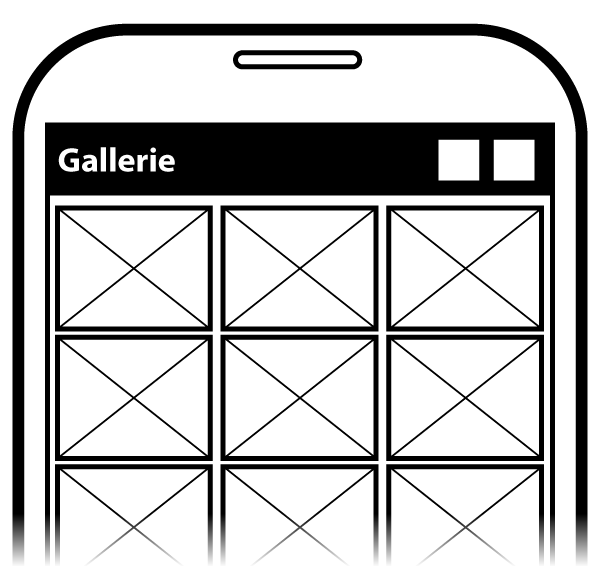
\includegraphics[width=0.49\textwidth]{img/software1_nohover.png}}
\hfill
\subfigure[Bildvergrößerung bei Annäherung]{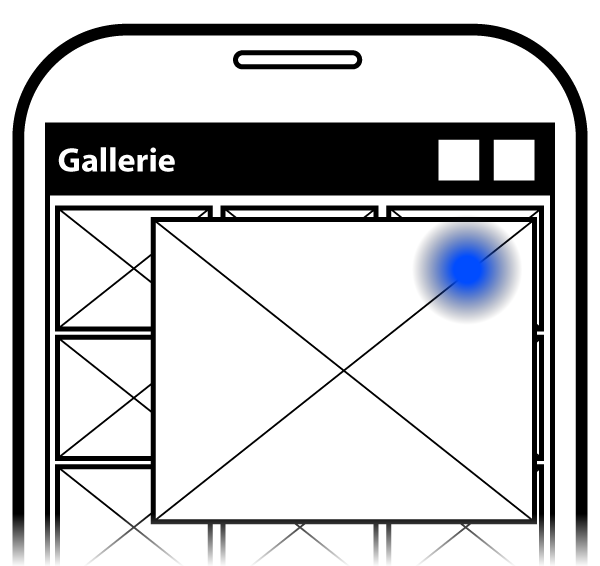
\includegraphics[width=0.49\textwidth]{img/software1_hover.png}}
\caption{Objektvergrößerungen bei Annäherung des Fingers mit aktiviertem AirView™ auf einem Samsung Galaxy S4.}
\label{samsungeinleitung1}
\end{figure}
Die zweite Art der Anwendungen zeigen bei Annäherung nicht Vergrößerungen oder detailliertere Ausführungen, sondern zuvor nicht sichtbare Informationen an. Somit können weitere Zusatzinformationen eingeblendet werden, siehe Abbildung \ref{samsungeinleitung2}. Als Beispiel dient der Wahlbildschirm, in der bei Annäherung auf eine aktive Kurzwahltaste der darauf jeweils gespeicherte Kurzwahlkontakt angezeigt wird.
\begin{figure}
\centering
\subfigure[Normalzustand des Wahlbildschirms]{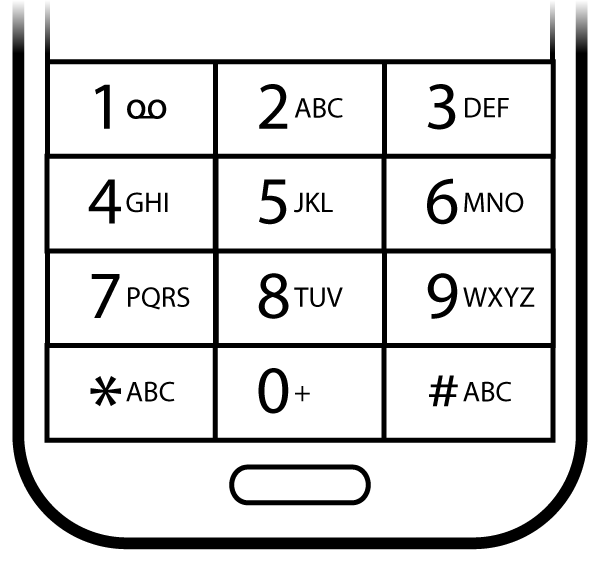
\includegraphics[width=0.49\textwidth]{img/software2_nohover.png}}
\hfill
\subfigure[Kurzwahlinformationen bei Annäherung]{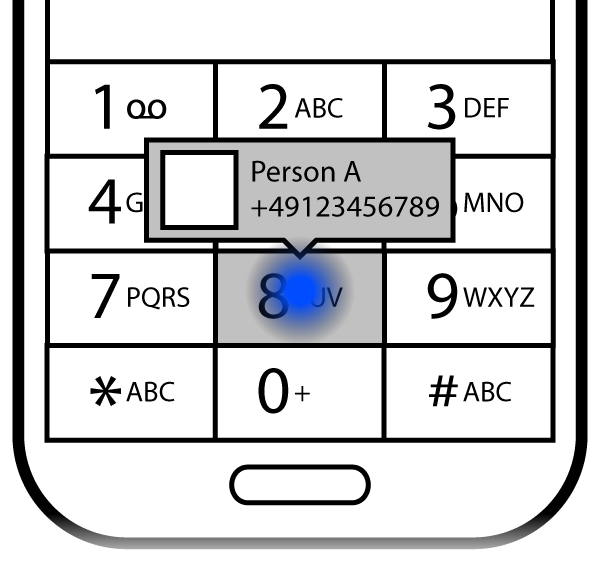
\includegraphics[width=0.49\textwidth]{img/software2_hover.png}}
\caption{Einblenden zusätzlicher Informationen bei Annäherung des Fingers auf einem Samsung Galaxy S4 mit aktiviertem AirView™.}
\label{samsungeinleitung2}
\end{figure}

\section{Bisherige Leitfäden für Bedienelemente}
Aufgrund der geringeren Abmessungen mobiler Endgeräte im Vergleich zu stationären Geräten und der direkten Bedienung mittels berührungsempfindlicher Bildschirme, ist die Gestaltung der Bedienelemente ein entscheidendes Kriterium für die reibungslose Interaktion zwischen Mensch und Maschine. Alle Hersteller der populären mobilen Betriebssysteme bieten umfangreiche Leitfäden an, die Empfehlungen für Anwendungsentwickler zur Gestaltung von Bedienelemente darstellen. In diesen Leitfäden werden u.A. Mindestangaben zu Größen und Abständen kommuniziert, siehe Tabelle \ref{leitfadenalle}. Wohingegen in Leitfäden für Desktop-Computer keine empfohlenen Mindestgrößen genannt werden.\\
Auch Studien zeigen, dass diese Leitfäden durchaus nötig sind. So arbeiten Nutzer mit Mausinteraktionen gegenüber Berührungsinteraktionen bisher präziser und schneller. Darüber hinaus wird die Interaktion mit der Maus bei Aufgaben, die genaue Selektionen benötigen, bevorzugt.\citep{touchmouse}
\begin{table}
\centering
\renewcommand{\arraystretch}{2}
\setlength{\tabcolsep}{15pt}
\begin{tabular}{ l c c }
Plattform & Minimale Größe & Empfohlene Größe\\\hline
Android \citep{androidrichtlinien} & 7mm & 9mm\\
Apple \citep{applerichtlinien} & 7mm & 7mm\\
Windows \citep{winrichtlinien} & 7mm & 9mm\\
\end{tabular}
\caption{Mindestgrößen von Bedienelementen.}
\label{leitfadenalle}
\end{table}
Aus diesen Gründen sollen die genannten Untersuchungen in dieser Bachelorarbeit auch prüfen, ob die Mindestgrößen unter Anwendung der Annäherungserkennung verkleinert werden können und die Präzision somit gesteigert werden kann.

\section{Lösungsansätze mittels Annäherungserkennung}
Durch die Annäherungserkennung werden Interaktionen auf einer weiteren Ebene ermöglicht und erweitern das Repertoire für den Designer einer Anwendung. Sony und Samsung haben mittlerweile Anwendungszenarios für die Annäherungserkennung demonstriert und damit gleichzeitig interessante Lösungen vorgestellt. Dieser Abschnitt soll diese Palette an Möglichkeiten erweitern und gleichzeitig den Bezug zu den behandelten Tests herstellen.

\subsection{Schaltflächenerkennung}\label{sec:schaltflächenerkennung}
Das Aussehen einer Schaltfläche variiert zwischen den unterschiedlichen Handymodellen, Betriebssystemen (z.B. iOS, Android) und Gerätetypen. Beispielsweise besitzen Schaltflächen auf einem mobilen Endgerät unter iOS andere Erscheinungsmerkmale als mobile Endgeräte unter Android. Dieser Umstand wird durch die Etablierung des Natural User Interfaces \citep{nui} verstärkt, da es die Abgrenzungen zu klassischen Schaltflächen aufweicht. Anstatt von Schaltflächen werden durch Wischgesten innerhalb bestimmter Bildschirmbereiche neue Aktionen ausgeführt. So werden mittlerweile für digitale Karten die klassischen Schaltflächen verstärkt durch Zoom- und Wischgesten ersetzt und ähneln damit der analogen Nutzung von Papierkarten.\\
Die Folge daraus könnten Schaltflächen sein, die für einzelne Nutzer nicht mehr als solche zu erkennen sind. Während auf Geräten mit Mausinteraktion die Listeneinträge bei Überlagerungen mit dem Mauszeiger hervorgehoben werden und damit als Schaltfläche erkennbar werden, fehlen diese Indikatoren bisher bei Bedienoberflächen für Geräte mit berührungsempfindlichen Bildschirmen. Die Annäherungserkennung könnte diese Lücke füllen und die aktuelle Fingerposition, ähnlich der Mauszeigerposition, in das Erscheinungsbild der Bedienoberfläche einbeziehen.
%Zudem müssen einige Nutzer dadurch nicht mehr mit der Befürchtung damit bereits eine Funktion auszulösen, den Bildschirm berühren, um anhand des darauffolgenden visuellem Feedback zu beurteilen, ob es sich an der Touchposition um eine Schaltfläche handelt.

\subsection{Tabellenhervorhebungen}
Durch die Annäherungserkennung bietet sich ein interessanter Lösungsansatz für eine mögliche Vereinfachung der visuellen Orientierung in vielspaltigen Tabellen an. Beim Suchen von einzelnen Einträgen in großen Tabellen ist bei manchen Nutzern zu beobachten, dass einzelne Zeilen mit dem Finger überfahren werden. Vielleicht könnte dieses Verhalten ausgenutzt werden, um den Nutzer in dieser Situation durch das Hervorheben ganzer Tabellenzeilen zu unterstützen. Im Rahmen dieser Bachelorarbeit wird eine derartige Tabellenhervorhebungen implementiert und getestet.

\subsection{Fingerpositionsmarkierungen}
In vielen Situationen kann es vorkommen, dass mehrere Schaltflächen auf engen Raum nebeneinander platziert sind, z.B. innerhalb unangepasster Webseiten auf kleinen Bildschirmen oder in Form von selektierbaren Straßenzügen oder Landesgrenzen in Kartenanwendungen bei großen Maßstäben. Durch die Annäherungserkennung ließe sich die aktuell durch den Finger überflogene Schaltfläche hervorheben (vgl. Abschnitt~\ref{sec:schaltflächenerkennung}) und dadurch eventuell die Selektierung durch den Nutzer vereinfachen. Eine mögliche Verbesserung der Usability durch Fingerpositionsmarkierungen soll im Rahmen dieser Bachelorarbeit überprüft werden.

\subsection{Vorhersage der Touchposition}
Als Ergänzung zur Fingerpositionsmarkierung wäre mittels der Annäherungserkennung eine Vorhersage der nachfolgenden Touchposition möglich, indem beispielsweise innerhalb eines definierten Radius die Schwebeposition des Fingers die Touchposition korrigiert. Schwebt der Finger eines Nutzer für eine Weile über eine sich hervorhebende Schaltfläche, so würde nach dieser Interpretation selbst eine anschließende, leicht verfehlte Berührung neben die Schaltfläche ausreichen, um diese auszulösen. Diese Ergänzung soll ebenfalls in einen der Tests dieser Bachelorarbeit evaluiert werden. Es ist dabei zu prüfen, ob somit die Genauigkeit auch bei kleinen Schaltflächen erhöht werden kann, die die Mindestgrößen laut der Leitfäden für Bedienelementen unterschreiten.

\chapter{Methodik}
In diesem Kapitel wird erläutert, wie die oben genannten Ansätze anhand von verschiedenen Usability-Tests überprüft werden.

\section{Testpersonen}
Die Testanwendung wurde in Usability-Tests von 18 Personen ausgiebig untersucht. Die Personen waren zwischen 20 und 35 Jahre alt (med: $23$ Jahre, \O: $25{,}\overline 5$ Jahre). Beide Geschlechter (8 weiblich, 10 männlich) waren ausgewogen am Test beteiligt. Das berufliche Umfeld der Testpersonen konzentrierte sich überwiegend auf den universitären Bereich. Zudem besaßen alle Testpersonen gute Erfahrungen in der Nutzung von Desktop-PCs, Laptops, Tablets oder Smartphones. Die dazugehörige Gewichtung im Bezug auf die Nutzung von Desktop-PCs, Laptops und anderen berührungsempfindlichen Geräten sind in Tabelle \ref{nutzungtestpersonen} dargestellt.
\begin{table}
\centering
\renewcommand{\arraystretch}{2}
\setlength{\tabcolsep}{4pt}
\begin{tabular}{ p{4.8cm} | c c c c c}
& Desktop-PC & Laptop & Tablet & Smartphone & Sonstige\\\hline
Weniger als 1x pro Monat & 50\% & 0\% & 59\% & 6\% & 56\%\\
Weniger als 1x pro Woche & 0\% & 6\% & 24\% & 0\% & 22\% \\
Weniger als 1x pro Tag & 17\% & 0\% & 12\% & 0\% & 17\% \\
Mehrmals am Tag & 33\% & 94\% & 6\% & 94\% & 6\% \\
\hline
Am häufigsten benutzt & 17\% & 44\% & 0\% & 39\% & 0\% \\
\end{tabular}
\caption{Gerätenutzung der Testpersonen.}
\label{nutzungtestpersonen}
\end{table}
Lediglich eine Person nahm innerhalb der letzten sechs Monate an Studien zu Interaktionen an Mobilgeräten oder an Studien der Digitalen Medien AG der Universität Bremen teil.

\section{Apparat}
Die Testumgebung besteht aus einem Testgerät und der zugehörigen für die Untersuchungen konzipierten Testanwendung.

Bei dem Testgerät handelt es sich um ein Samsung Galaxy S4. Das darauf installierte Betriebssystem basiert auf Android in der Version 4.4 (API-Level: 19). Der kapazitive Touchscreen des Smartphones mit einer Bildschirmdiagonalen von 5 Zoll besitzt eine Auflösung von 1920$\times$1080 Pixeln und unterstützt die Annäherungserkennung. Das Smartphone darf während der Tests von den Testpersonen festgehalten, jedoch nicht von der Tischfläche angehoben werden.

Die Testumgebung beinhaltet als zweite Komponente die Testanwendung, die den Testpersonen unterschiedliche Aufgaben stellt. Die Testanwendung wurde in Java entwickelt und eigens für das Samsung Galaxy S4 konzipiert. Dazu wurde zudem die Bedienoberfläche der Testanwendung auf die entsprechende Bildschirmgröße angepasst und die von Samsung dokumentierte API für AirView™ in die Testanwendung integriert. Schließlich wurde die Testanwendung mittels des Android-SDKs in Version 19 kompiliert und auf das Gerät installiert. Der Quelltext liegt in digitaler Form auf dem beiliegenden Datenträger dieser Bachelorarbeit vor. Zusätzlich wird an dieser Stelle auch eine installierbare APK-Datei zur Verfügung gestellt.\\
Innerhalb der Testanwendung wird zu Beginn jeder Testsitzung eine Identifikationsnummer angezeigt, die für die jeweilige Testsitzung bestimmt wurde. Während jeder Testsitzung werden von der Testanwendung alle relevanten Interaktionen des Nutzers protokolliert und mit der zugehörigen Identifikationsnummer in eine auf dem Gerät angelegten Textdatei gespeichert.\\
Die Testanwendung ist in zwei unterschiedliche Tests unterteilt und wurde so gestaltet, dass vor jedem Testbeginn eine entsprechende Testbeschreibung angezeigt wird, siehe Abbildung \ref{apparattestbeschreibung}.
\begin{figure}
\centering
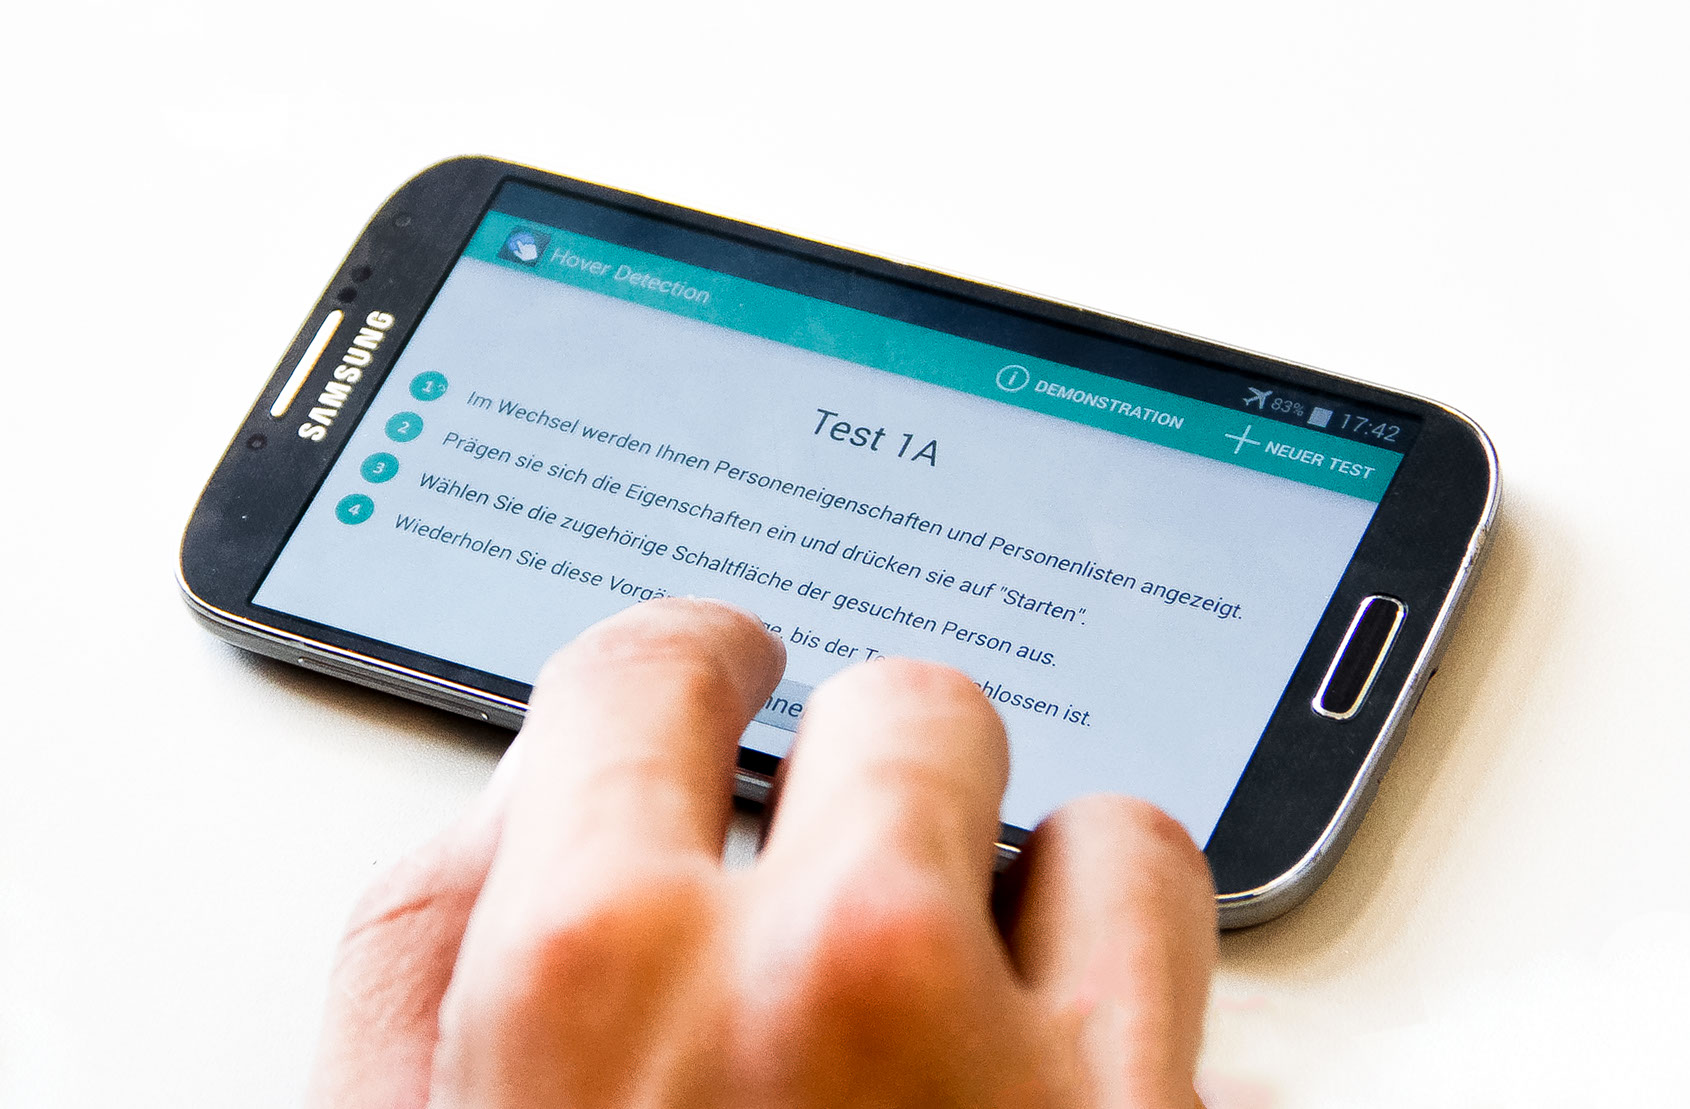
\includegraphics[width=0.68\textwidth]{img/apparatus1.jpg}
\caption{Testbeschreibung des ersten Tests.}
\label{apparattestbeschreibung}
\end{figure}

\subsection{Test 1: Listenauswahl}
\begin{figure}
\centering
\subfigure[Phase 1: Zu suchende Person wird beschrieben.]{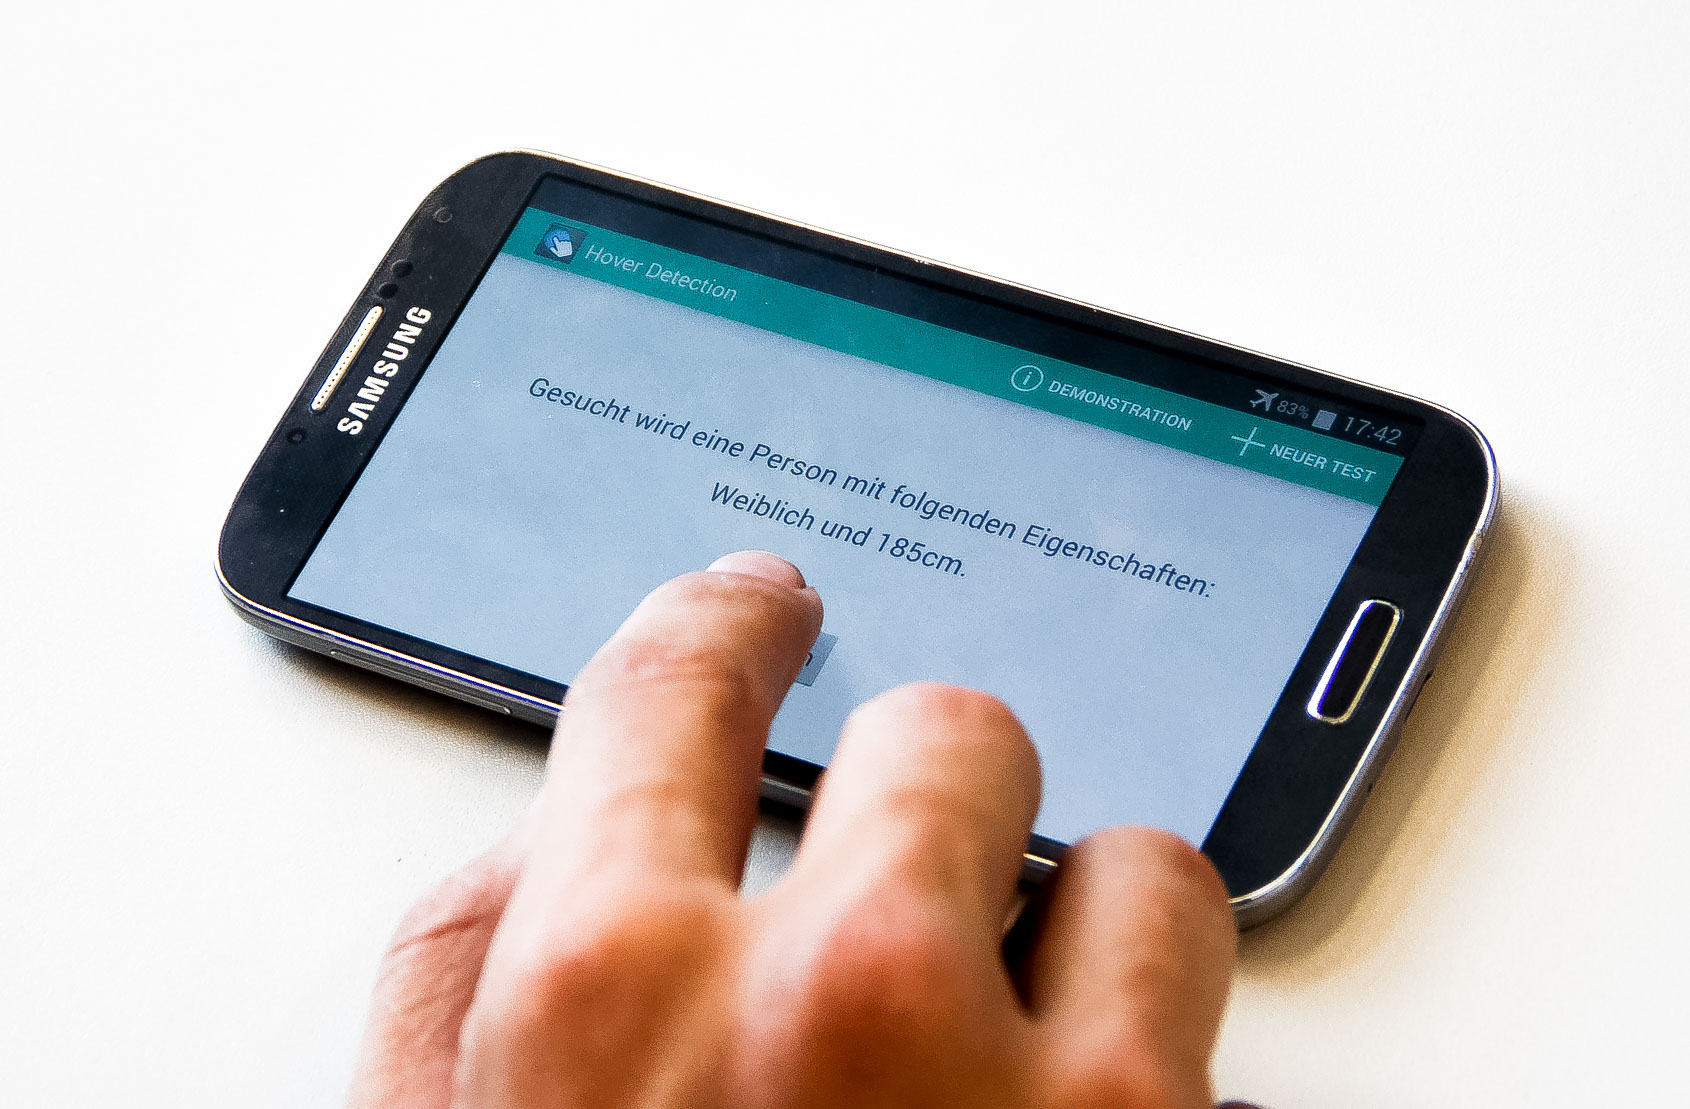
\includegraphics[width=0.68\textwidth]{img/test1_phase1.jpg}}
\subfigure[Phase 2: Anzeige einer pseudozufälligen Personenliste.]{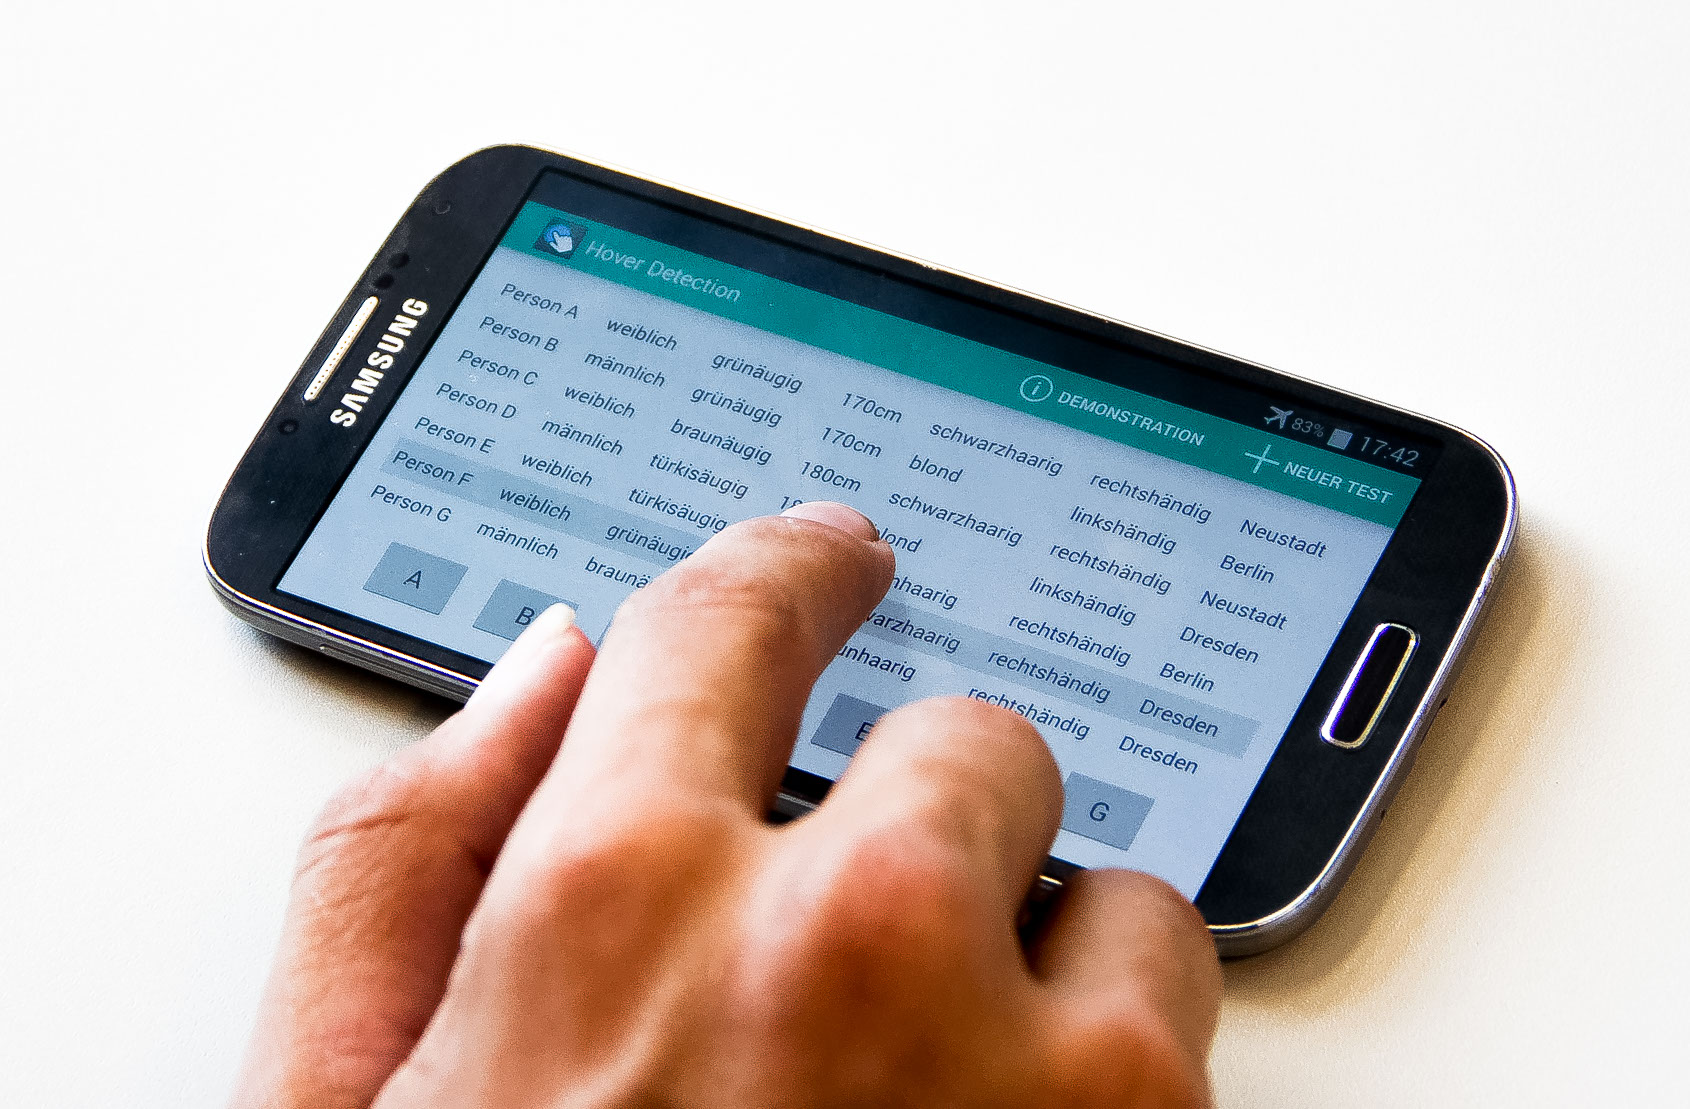
\includegraphics[width=0.68\textwidth]{img/test1_phase2.jpg}}
\subfigure[Phase 3: Gesuchte Person in der unteren Leiste auswählen.]{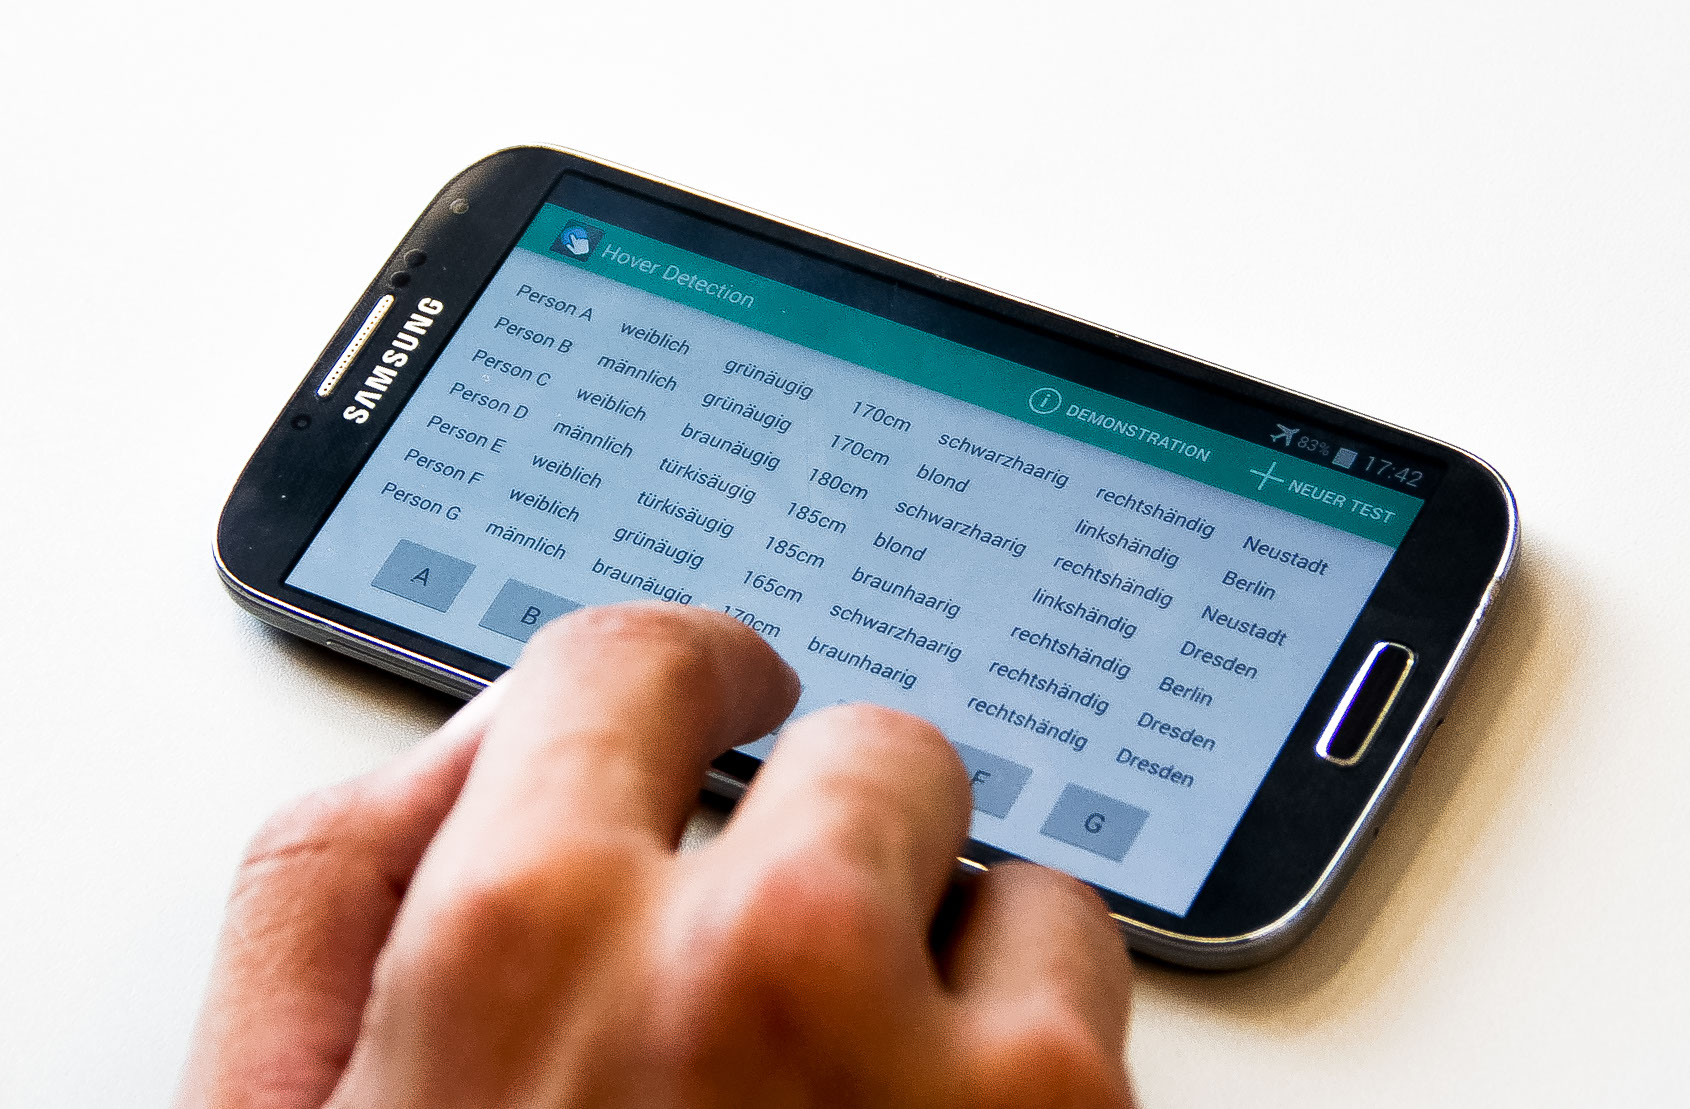
\includegraphics[width=0.68\textwidth]{img/test1_phase3.jpg}}
\caption{Aufbau von Test 1: Drei unterschiedliche Phasen pro Durchgang.}
\label{test1phasen}
\end{figure}
Die Testanwendung ermöglicht im ersten Test, die Wirkung von Hervorhebungen der Listeneinträge bei Annäherung zu überprüfen, siehe Abbildung \ref{test1phasen}.\\
Hierzu wird dem Nutzer ein Anweisungsbildschirm mit zwei pseudozufälligen Personeneigenschaften eingeblendet. Nachdem der Nutzer sich die Eigenschaften eingeprägt und anschließend auf "`Starten"' gedrückt hat, wird eine mehrspaltige Personenliste mit sieben fiktiven Personen und ihren Eigenschaften angezeigt. Nähert sich der Finger des Nutzers nun einem Listeneintrag, so wird dieser hervorgehoben. Der Test ist so aufgebaut, dass pro Anweisung nur exakt eine Person die gesuchten Eigenschaften besitzt. Der Nutzer hat anschließend eine korrekte Person auszuwählen, indem dabei die Schaltfläche mit dem entsprechenden Personenname (Buchstaben von A-G) berührt wird. Sollte die falsche Schaltfläche berührt werden, so wird der Nutzer mittels einer temporären Texteinblendung (konkret: "`Toast-Notification"') über die Falschberührung informiert und erneut an die zu suchende Eigenschaften erinnert. War die Personenauswahl korrekt, so werden dem Nutzer in weiteren Runden neue Eigenschaften auf dem Anweisungsbildschirm angezeigt. Der Test ist beendet, sobald der Nutzer sieben unterschiedliche Anweisungen befolgt hat.

Um zu überprüfen, ob die Hervorhebungen der Listeneinträge bei Annäherungen einen Einfluss auf die Aufgabenerfüllung gehabt haben, wird der Test ein zweites Mal wiederholt. Bei der Wiederholung wird je nach Testvariante dann die Annäherungserkennung zu- oder abgeschaltet.

\subsection{Test 2: Präzisionstest}
\begin{figure}
\centering
\subfigure[Phase 1: Halten der grünen Schaltfläche.]{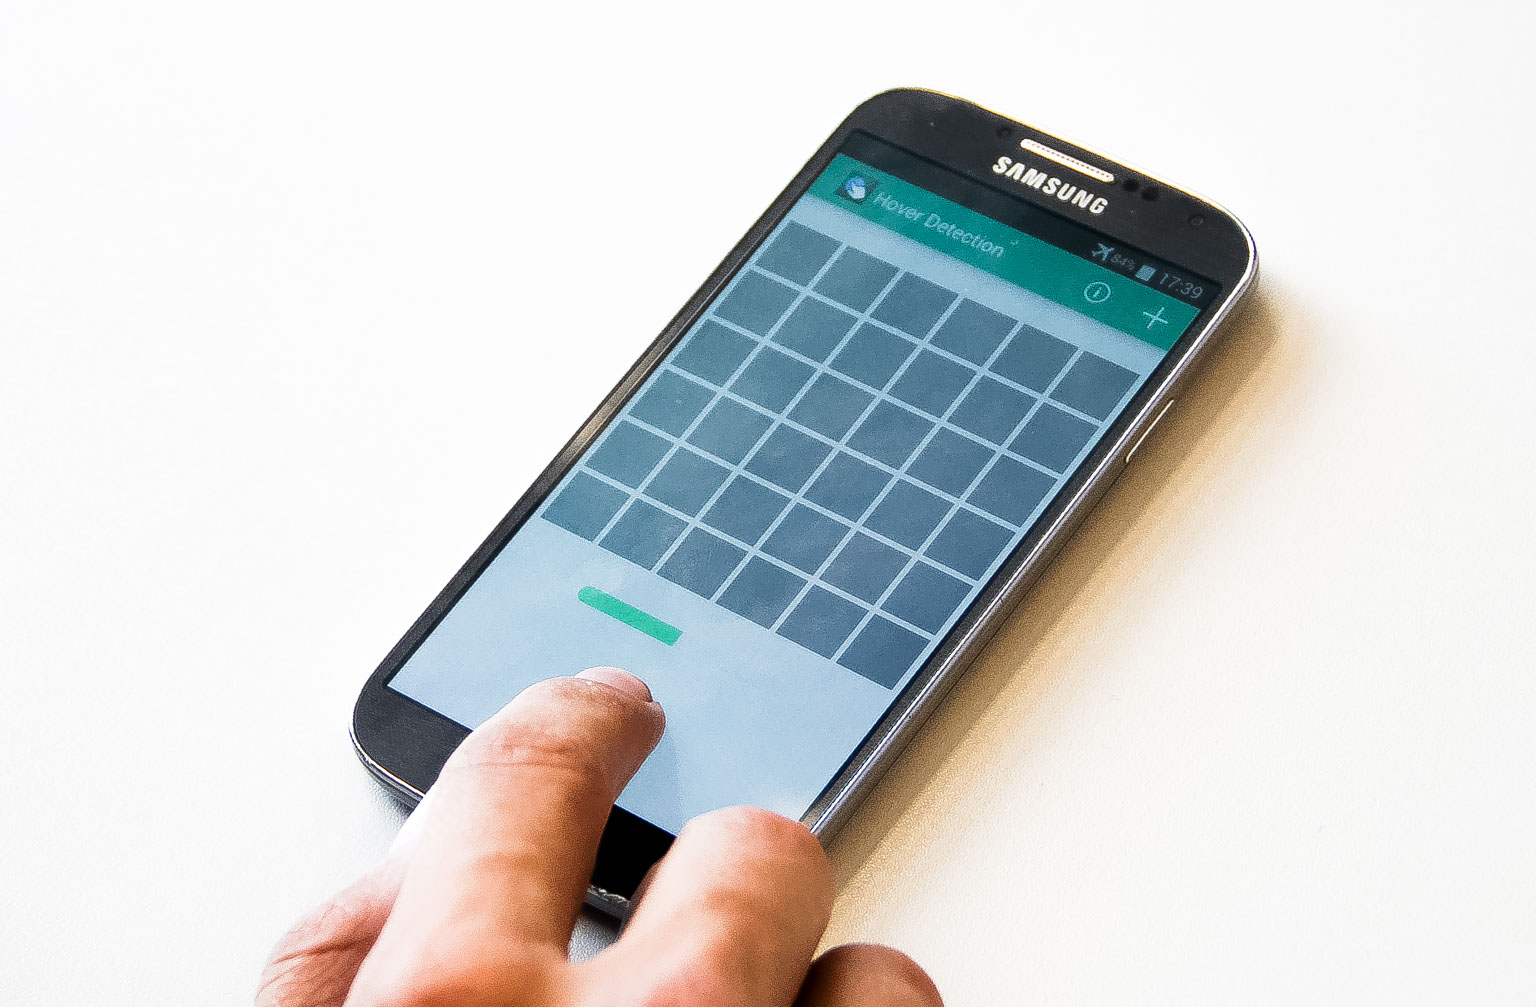
\includegraphics[width=0.68\textwidth]{img/test2_phase1.jpg}}
\subfigure[Phase 2: Blaue Schaltfläche leuchtet pseudozufällig auf.]{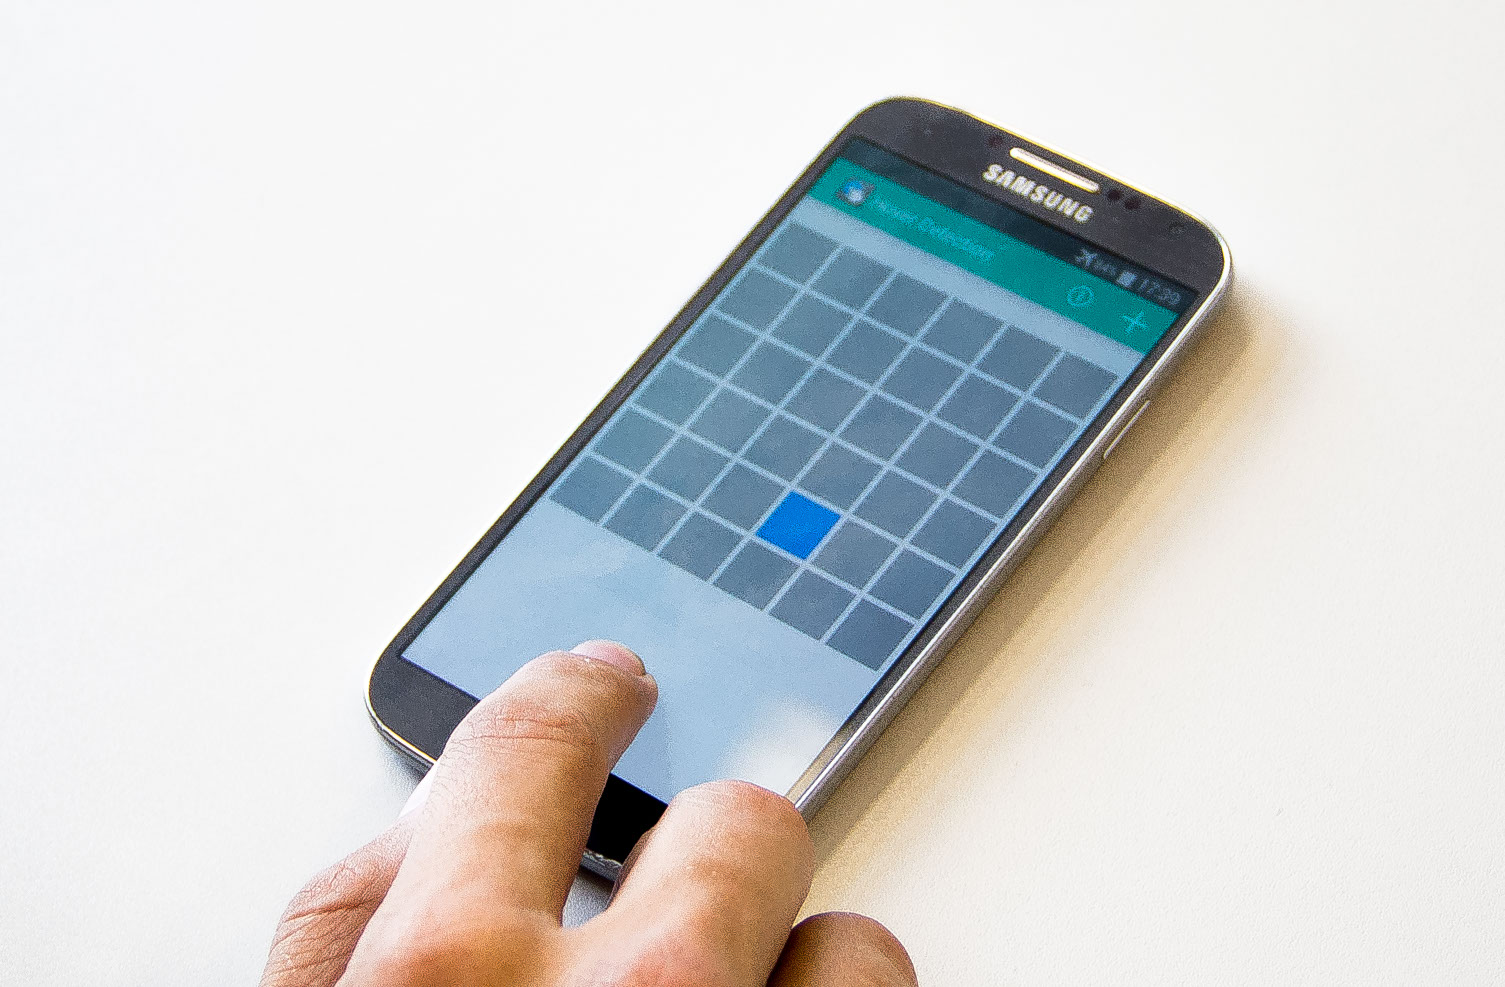
\includegraphics[width=0.68\textwidth]{img/test2_phase2.jpg}}
\subfigure[Phase 3: Berühren der blauen Schaltfläche.]{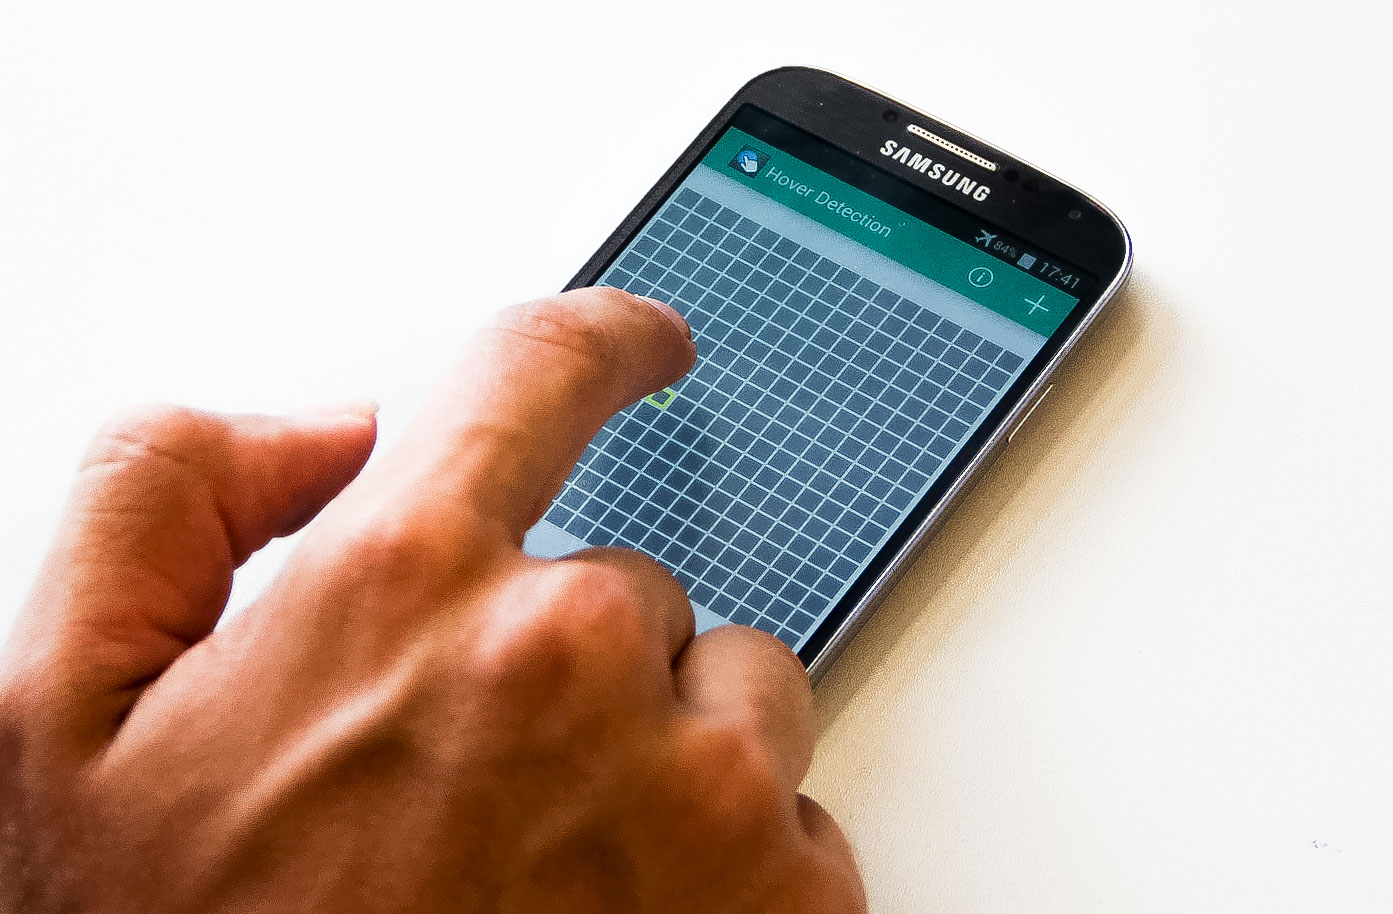
\includegraphics[width=0.68\textwidth]{img/test2_phase3.jpg}}
\caption{Aufbau von Test 2: Drei unterschiedliche Phasen pro Durchgang.}
\label{test2phasen}
\end{figure}
Die Testanwendung ermöglicht im zweiten Test, die Wirkung von Hervorhebungen auf die empfohlene Mindestgröße von Bedienelementen zu überprüfen, siehe Abbildung \ref{test2phasen}.\\
Die Bedienoberfläche zeigt einen Anweisungstext an, die den Nutzer auf das Halten der grünen, runden Schaltfläche am unteren Bildschirmrand hinweist. Um diese Schaltfläche zu halten, muss diese berührt und der Finger nicht angehoben werden. Anschließend läuft für eineinhalb Sekunden ein Fortschrittsbalken ab. Die Testanwendung blendet im nächsten Schritt ein quadratisches Gitter mit quadratischen, grauen Schaltflächen ein. Eine graue Schaltfläche wird pseudozufällig von der Testanwendung ausgewählt und blau koloriert. Der Nutzer hat diese Schaltfläche im Anschluss zu berühren. Ist die Annäherungserkennung aktiviert, wird diejenige Schaltfläche aktiviert, die die momentane Fingerschwebepostion überspannt. Wird nun der Bildschirm berührt, so wird dem Nutzer über die Einblendung eines Anweisungsbildschirms die erfolgreiche oder misslungene Berührung mitgeteilt. Die Berührung gilt als erfolgreich, wenn die blaue Schaltfläche als erstes berührt worden ist.
Ist die Berührung misslungen, so wird die Kolorierung solange zurückgesetzt, bis der Nutzer die grüne Schaltfläche erneut und für eine zusätzliche Sekunde gehalten hat. Der Nutzer hat anschließend vier weitere Versuche, um die blaue Schaltfläche zu treffen, andernfalls wird der Test vorläufig beendet.
Neben den bereits erwähnten Benachrichtigungen, wird bei einer erfolgreichen Berührung dem Nutzer die Erhöhung des Schwierigkeitsgrades signalisiert. Gleichzeitig wird die grüne Schaltfläche wieder am unteren Bildschirmrand eingeblendet und der Nutzer kann den Test im nächsten Schwierigkeitsgrad fortsetzen. Der Test wird beendet, sobald alle Schwierigkeitsgrade von Nutzer bewältigt worden sind.

Die Testanwendung ist so konzipiert, dass beliebig viele Schwierigkeitsgrade und Schaltflächengrößen getestet werden können. Die Größe der Schaltfläche kann für jeden Schwierigkeitsgrad individuell angepasst werden. Die Testanwendung ist so gestaltet, dass neben dem obligatorischen Zeitpunkt der Interaktion sowohl die Position der grünen und blauen Schaltflächen auf dem Bildschirm, als auch die genauen Berührungspunkte auf diesen Schaltflächen selbst protokolliert werden. Im Falle einer eventuelle Formelanwendung nach Fitts \citep{fitts} sind somit alle Parameter für jeden Versuch und Schwierigkeitsgrad vorhanden oder kalkulierbar.

Um auch in diesem Test die Auswirkungen der Annäherungserkennung zu untersuchen, wird dieser Test ebenfalls wiederholt. Dieser Test benötigt aufgrund der drei Testvarianten zwei Wiederholungen. Während einer Wiederholung werden die Hervorhebungen zu- oder abgeschaltet, in der anderen die softwareseitige Selektionshilfe.

Die softwareseitige Selektionshilfe manipuliert dabei die Eingabe des Nutzers. Anstatt die tatsächliche Berührungspostions des Fingers zu berücksichtigen, wird die Schwebeposition der Annäherungserkennung verwendet. Diese Manipulation wird jedoch nur getätigt, wenn der Positionsunterschied der Schwebe- und Berührungsposition XXmm unterschreitet.

\subsection{Ausbalancieren von Gewöhnungseffekten}
Damit alle erhobenen Messwerte, u.A. die Auswahlgeschwindigkeiten, nicht durch etwaige Gewöhnungen während vorhergehende Testdurchgänge verfälscht werden und dies die statistische Auswertung verfälschen würde, muss die Reihenfolge auf die Testteilnehmer gleichmäßig variiert werden.\\
Hierzu sind die Testpersonen gemäß des Latin Squares in unterschiedliche Gruppen einzuteilen. Aus diesem Grund wurde bei der Konzeption der Testanwendung darauf geachtet, dass die Tests in unterschiedlichen Reihenfolgen gestartet werden können.\\
Zudem ist die Reihenfolge der Ereignisse in jedem einzelnen Test pseudozufällig, d.h. aus Sicht des Nutzers rein zufällig, ausgewählt worden. Tatsächlich durchläuft jeder Nutzer in einer bestimmten Gruppe jedoch die exakt gleichen Aufgaben. Dies soll sicherstellen, dass etwaige Gewöhnungen auch gleichmäßig auf die Testvarianten aufgeteilt werden.\\
Beispielweise wird im ersten Test jede Testvariante gleichmäßig auf die erste, zweite oder dritte Wiederholung gelegt. Gleichzeitig werden dadurch die Anweisungen aufgrund ihrer fixen Reihenfolge auf jede Testvariante ausgeglichen verteilt. Der selbe Ansatz wird für die Personenliste genutzt: Entsprechend der Anweisung werden den Personen andere Eigenschaften zugeordnet. Dementsprechend ist auch im zweiten Test die Positionsreihenfolge der blauen Zielschaltflächen an die jeweilige Schaltflächengröße gekoppelt. Somit werden auch im zweiten Test alle Positionen gleichmäßig von jeder Testvariante verwendet.

\subsection{Kalibrierung der Annäherungserkennung}
Während der Implementierungsphase der Testanwendung konnten im Bezug auf die ermittelte Schwebeposition des Fingers auffallende  Verschiebungen zur tatsächlichen Fingerposition beobachtet werden. Es war somit anzunehmen, dass bei der Annäherungserkennung noch bestehende Ungenauigkeiten vorliegen. Weiterhin kann je nach Anstellwinkel des Fingers der dichteste Punkt zum Bildschirm variieren und dies möglicherweise eine zusätzliche Ungenauigkeit zur Folge haben. Beim internen Testen der Testanwendung zeigten sich teilweise deutliche Unterschiede zwischen den Schwebe- und Touchpositionen. Resultierend daraus wurden die kleinen Quadrate im zweiten Test unter Umständen nicht mehr korrekt hervorgehoben, bevor diese schließlich berührt werden würden.

Um die Verschiebungen zwischen der Schwebe- und Touchposition des Fingers nachzuvollziehen, wurde der Testanwendung eine optional zuschaltbare Ebene innerhalb der Benutzungsoberfläche hinzugefügt, die die letzte Touch- und Schwebeposition anhand von Kreuzen sichtbar machte. Bei internen Versuchen mit der Testanwendung wurde deutlich, dass in bestimmten Bereichen die beiden Kreuze nicht aufeinander lagen und die Touch- und Schwebeposition sich somit unterschiedlich stark unterschieden.

Um mögliche Zusammenhänge der Verschiebungen zwischen der Touch- und Schwebeposition des Fingers nachzuweisen, wurde eine Testanwendung implementiert, die die letzte Schwebe- und Touchposition aufzeichnete. Dabei sollten Nutzer eine Abfolge von verschiedenen Punkte auf dem Bildschirm berühren. Die jeweiligen Schwebe- und Touchpositionen waren für die Testperson zu diesem Zeitpunkt nicht sichtbar und wurden erst nach dem eigentlichen Test visualisiert.
\begin{figure}
\centering
\subfigure[Interaktion mit dem Finger]{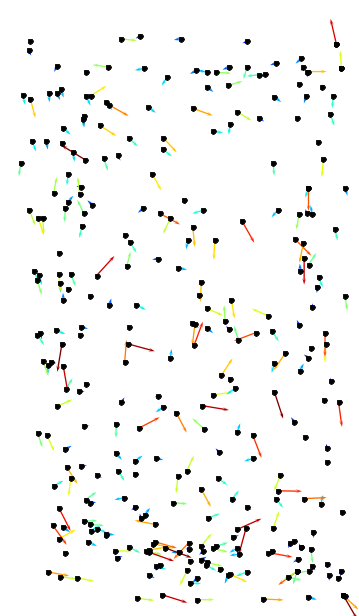
\includegraphics[width=0.45\textwidth]{img/kalibrierung1_finger.png}}
\hfill
\subfigure[Interaktion mit dem Daumen]{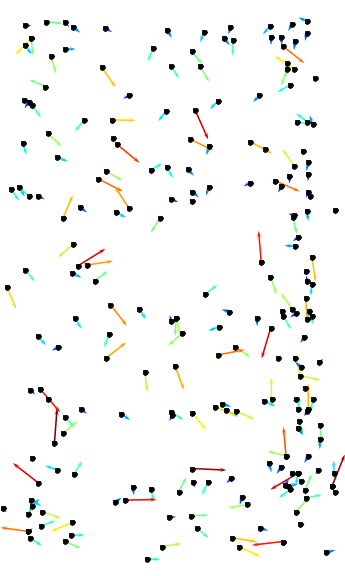
\includegraphics[width=0.45\textwidth]{img/kalibrierung1_daumen.png}}
\caption{Visualisierung der relativen Verschiebungen zwischen der Touch- und Schwebeposition. Die Pfeile inkl. Farbtemperatur deuten die Distanz der Verschiebung an.}
\label{klickschwebepositionen}
\end{figure}
Anschließend wurden die Werte mittels eines eigens geschriebenen Hilfsprogramm ausgewertet und visualisiert.

Die Abbildung \ref{klickschwebepositionen} zeigt die relativen Verschiebungen zwischen der Touch- und Schwebeposition an und verdeutlicht gleichzeitig die teilweise sehr starken Schwankungen beider Werte. Obwohl an mehreren stellen Tendenzen zur Verschiebungsrichtung erkennbar sind, besitzen die Werte dennoch eine große Streuung. Die Möglichkeit, die Schwebepositionen auf die Touchpositionen zu verschieben (und andersherum), wären theoretisch möglich, z.B. durch lineare oder polynominale Regression. Da die Ermittlung dieser Variablen den Umfang dieser Bachelorarbeit jedoch überstiegen hätte, wurde eine Kalibrierung im Rahmen dieses Tests nicht verfolgt. Stattdessen wurde für den zweiten Tests eine weitere Testvariante mit aktivierter Selektionshilfe implementiert.

\subsection{Fragebögen}
Um für die spätere Auswertung genügend Informationen über die jeweiligen Testpersonen zu erhalten, sollen jeder Testperson mehrere Fragebögen ausgehändigt werden.

\subsubsection{Personenfragebogen}
Allgemeine Personeninformationen, wie Alter und Berufsfeld, ermöglichen es, die jeweilige Testpersonen in Personengruppen einzuordnen. Dies ist beispielsweise sinnvoll, sobald sich im Bezug auf die Testergebnisse signifikante Unterschiede zwischen den verschiedenen Personengruppen ergeben. Aus diesem Grund wurde für die Studie ein Personenfragebogen angefertigt, siehe Anhang \ref{lab:Personenfragebogen}.\\
Zusätzlich wird nach der Sehstärke, während der Testsitzung getragene Sehhilfen und den Erfahrungen mit berührungsempfindlichen Bildschirmen gefragt. Durch diese Daten können etwaige Probleme während der Testsitzung erklärt werden, z.B. schlechtes Abschneiden durch ungenügende Sehschärfe oder mangelnder Erfahrung.\\
Damit der Testleiter mögliche Störeinflüsse während des Tests aufnehmen kann, verfügt der Personenfragebogen zusätzlich über ein entsprechendes Textfeld.

\subsubsection{System Usability Scale}
Der System Usability Scale \citep{sus} ist eine verbreitete Möglichkeit die Usability eines Systems zu testen. Somit kann diese sowohl allgemein eingeordnet, als auch für jeden Test einzeln verglichen werden. Dies setzt voraus, dass für jeden Test und der dazugehörigen Testvariante ein System Usability Scale angefertigt wird, siehe Anhang \ref{lab:Bewertungsbögen}.

\subsubsection{Qualitativer Fragebogen}
Der qualitative Fragebogen bestehend aus überwiegend frei beantwortbaren Fragen, soll die positiven und negativen Gedanken erfassen, die die Testperson mittels des System Usability Scales nicht erfassen konnte. Auch Verbesserungsvorschläge oder sonstige Anmerkungen der Testperson können hier aufgenommen werden. Zusätzlich werden die Testpersonen für den Ausblick nach mögliche Anwendungsgebieten gefragt, siehe Anhang \ref{lab:Bewertungsbögen}.

\section{Prozedur}
\begin{figure}
\centering
\subfigure[Räumlichkeiten der Testsitzung]{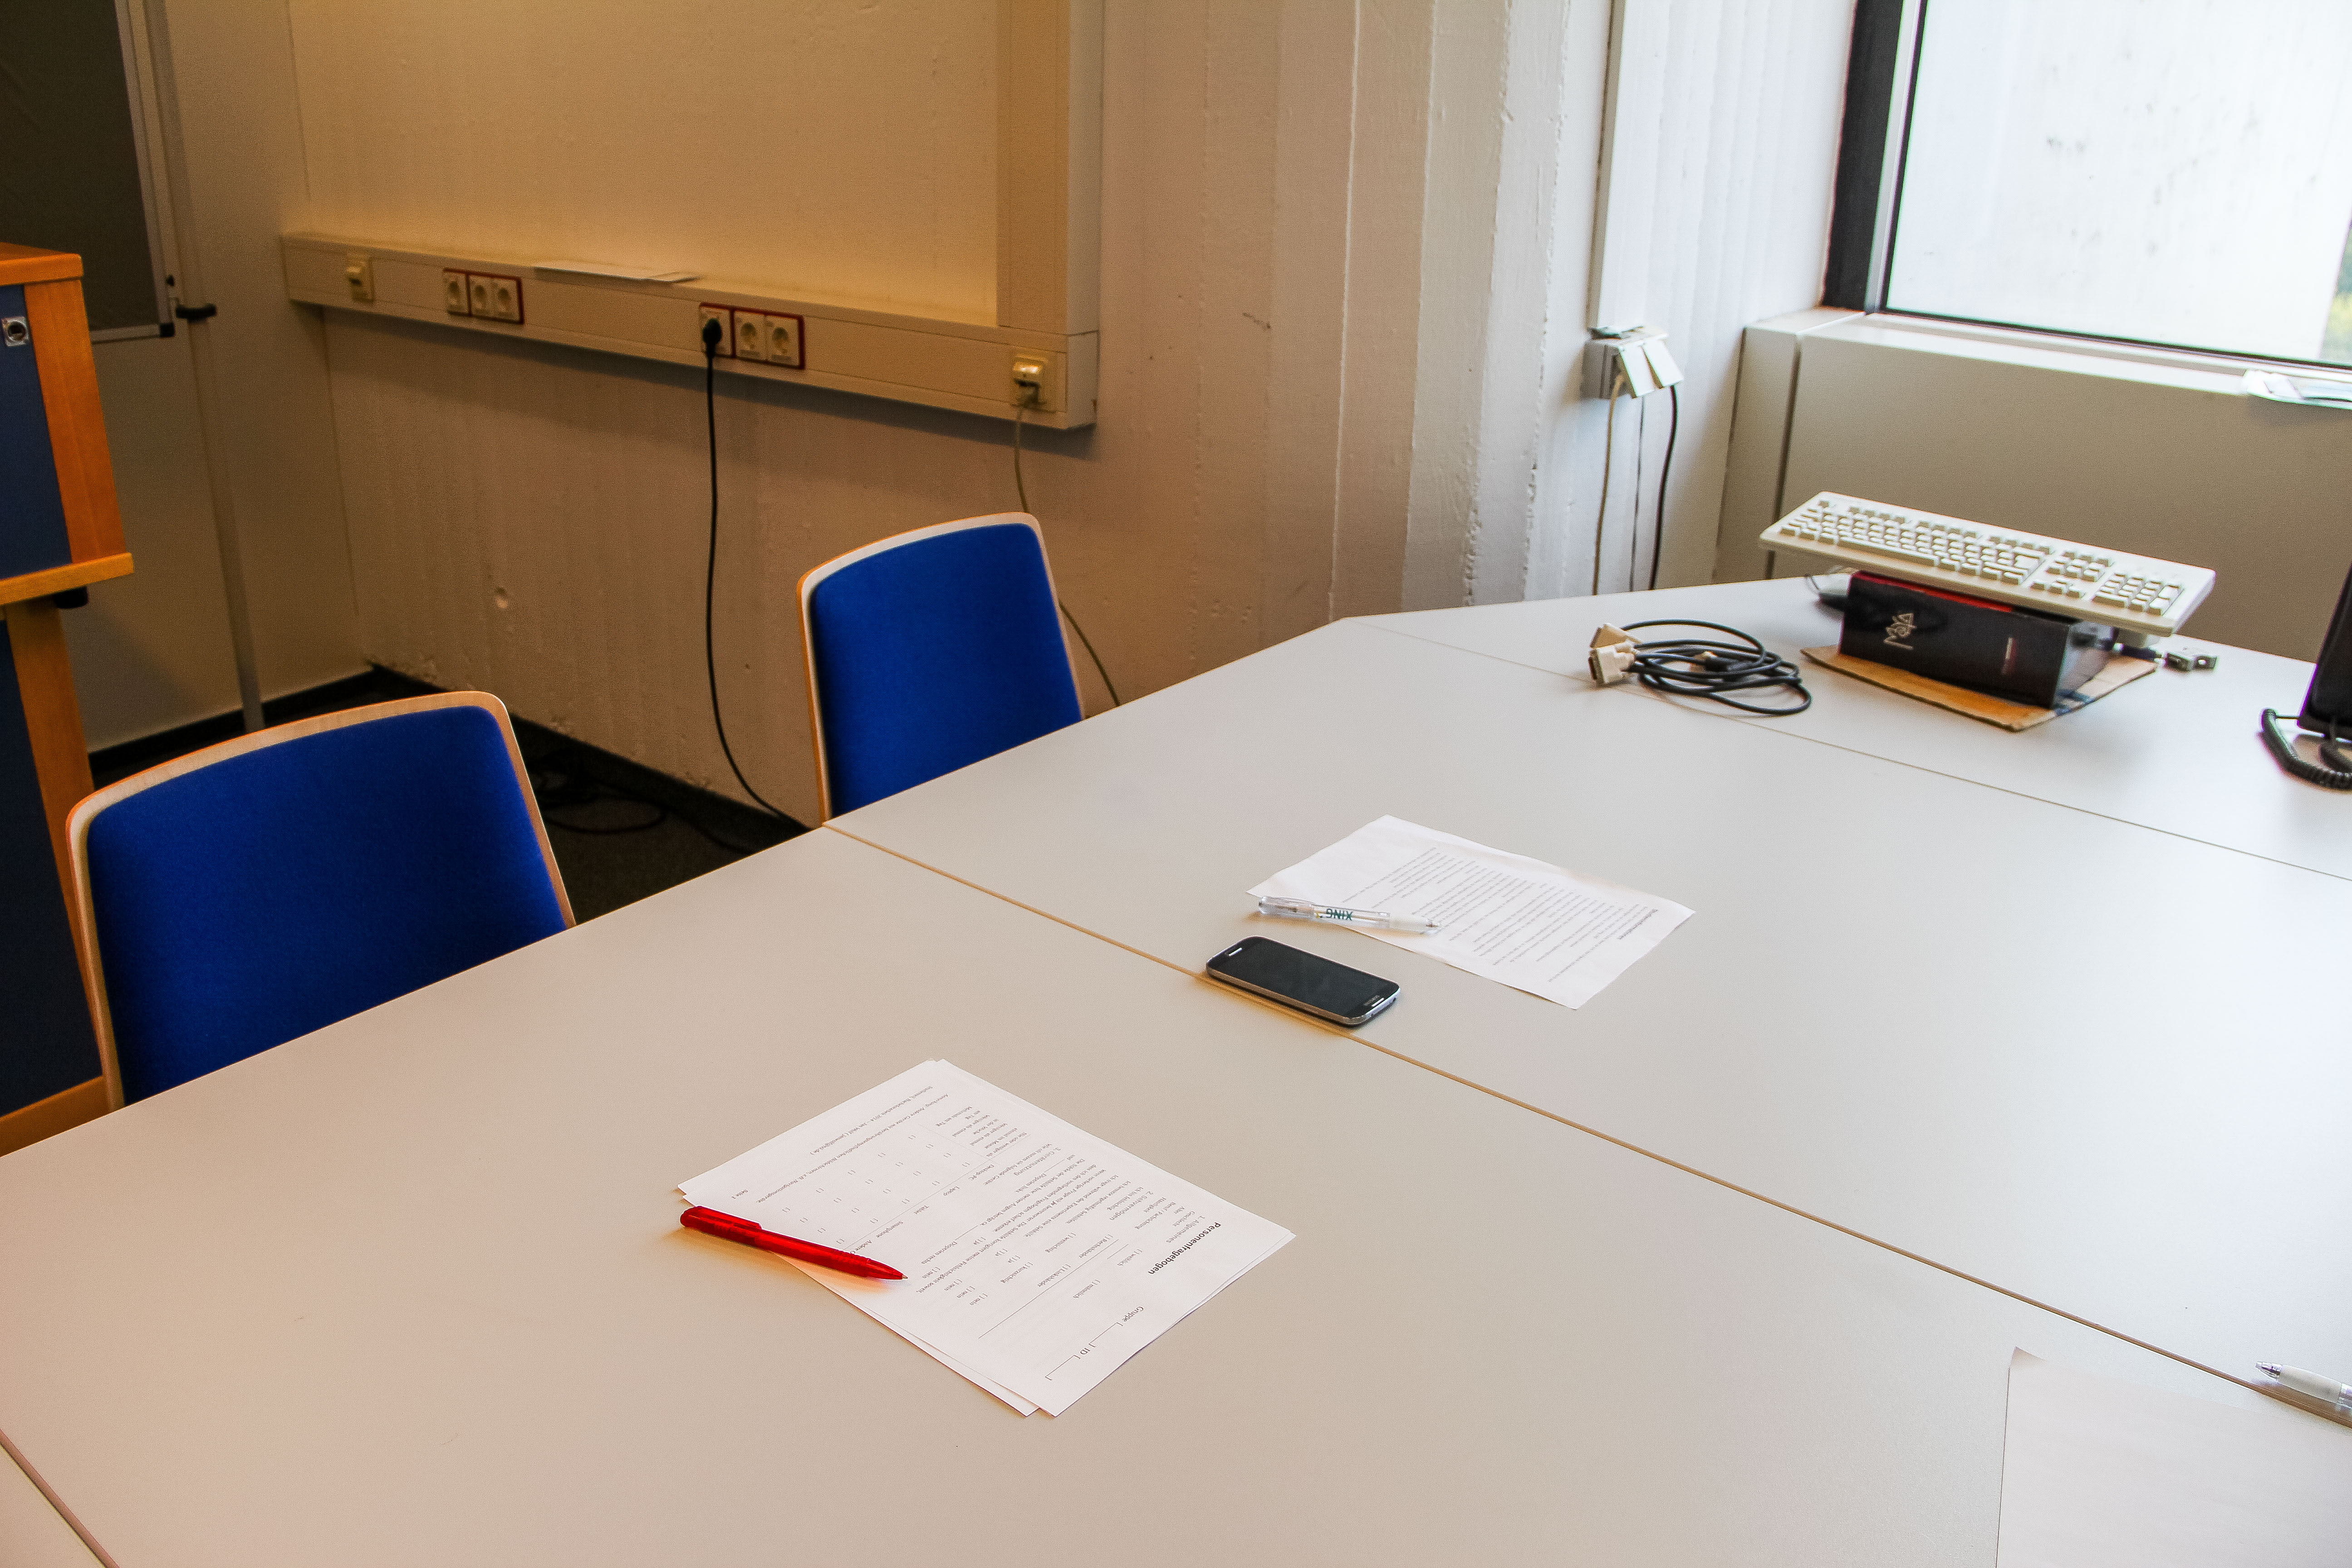
\includegraphics[width=0.67\textwidth]{img/prozedur1.jpg}}
\subfigure[Testumgebung und Fragebögen]{\includegraphics[width=0.67\textwidth]{img/prozedur2.jpg}}
\subfigure[Testperson füllt Personenfragebogen aus]{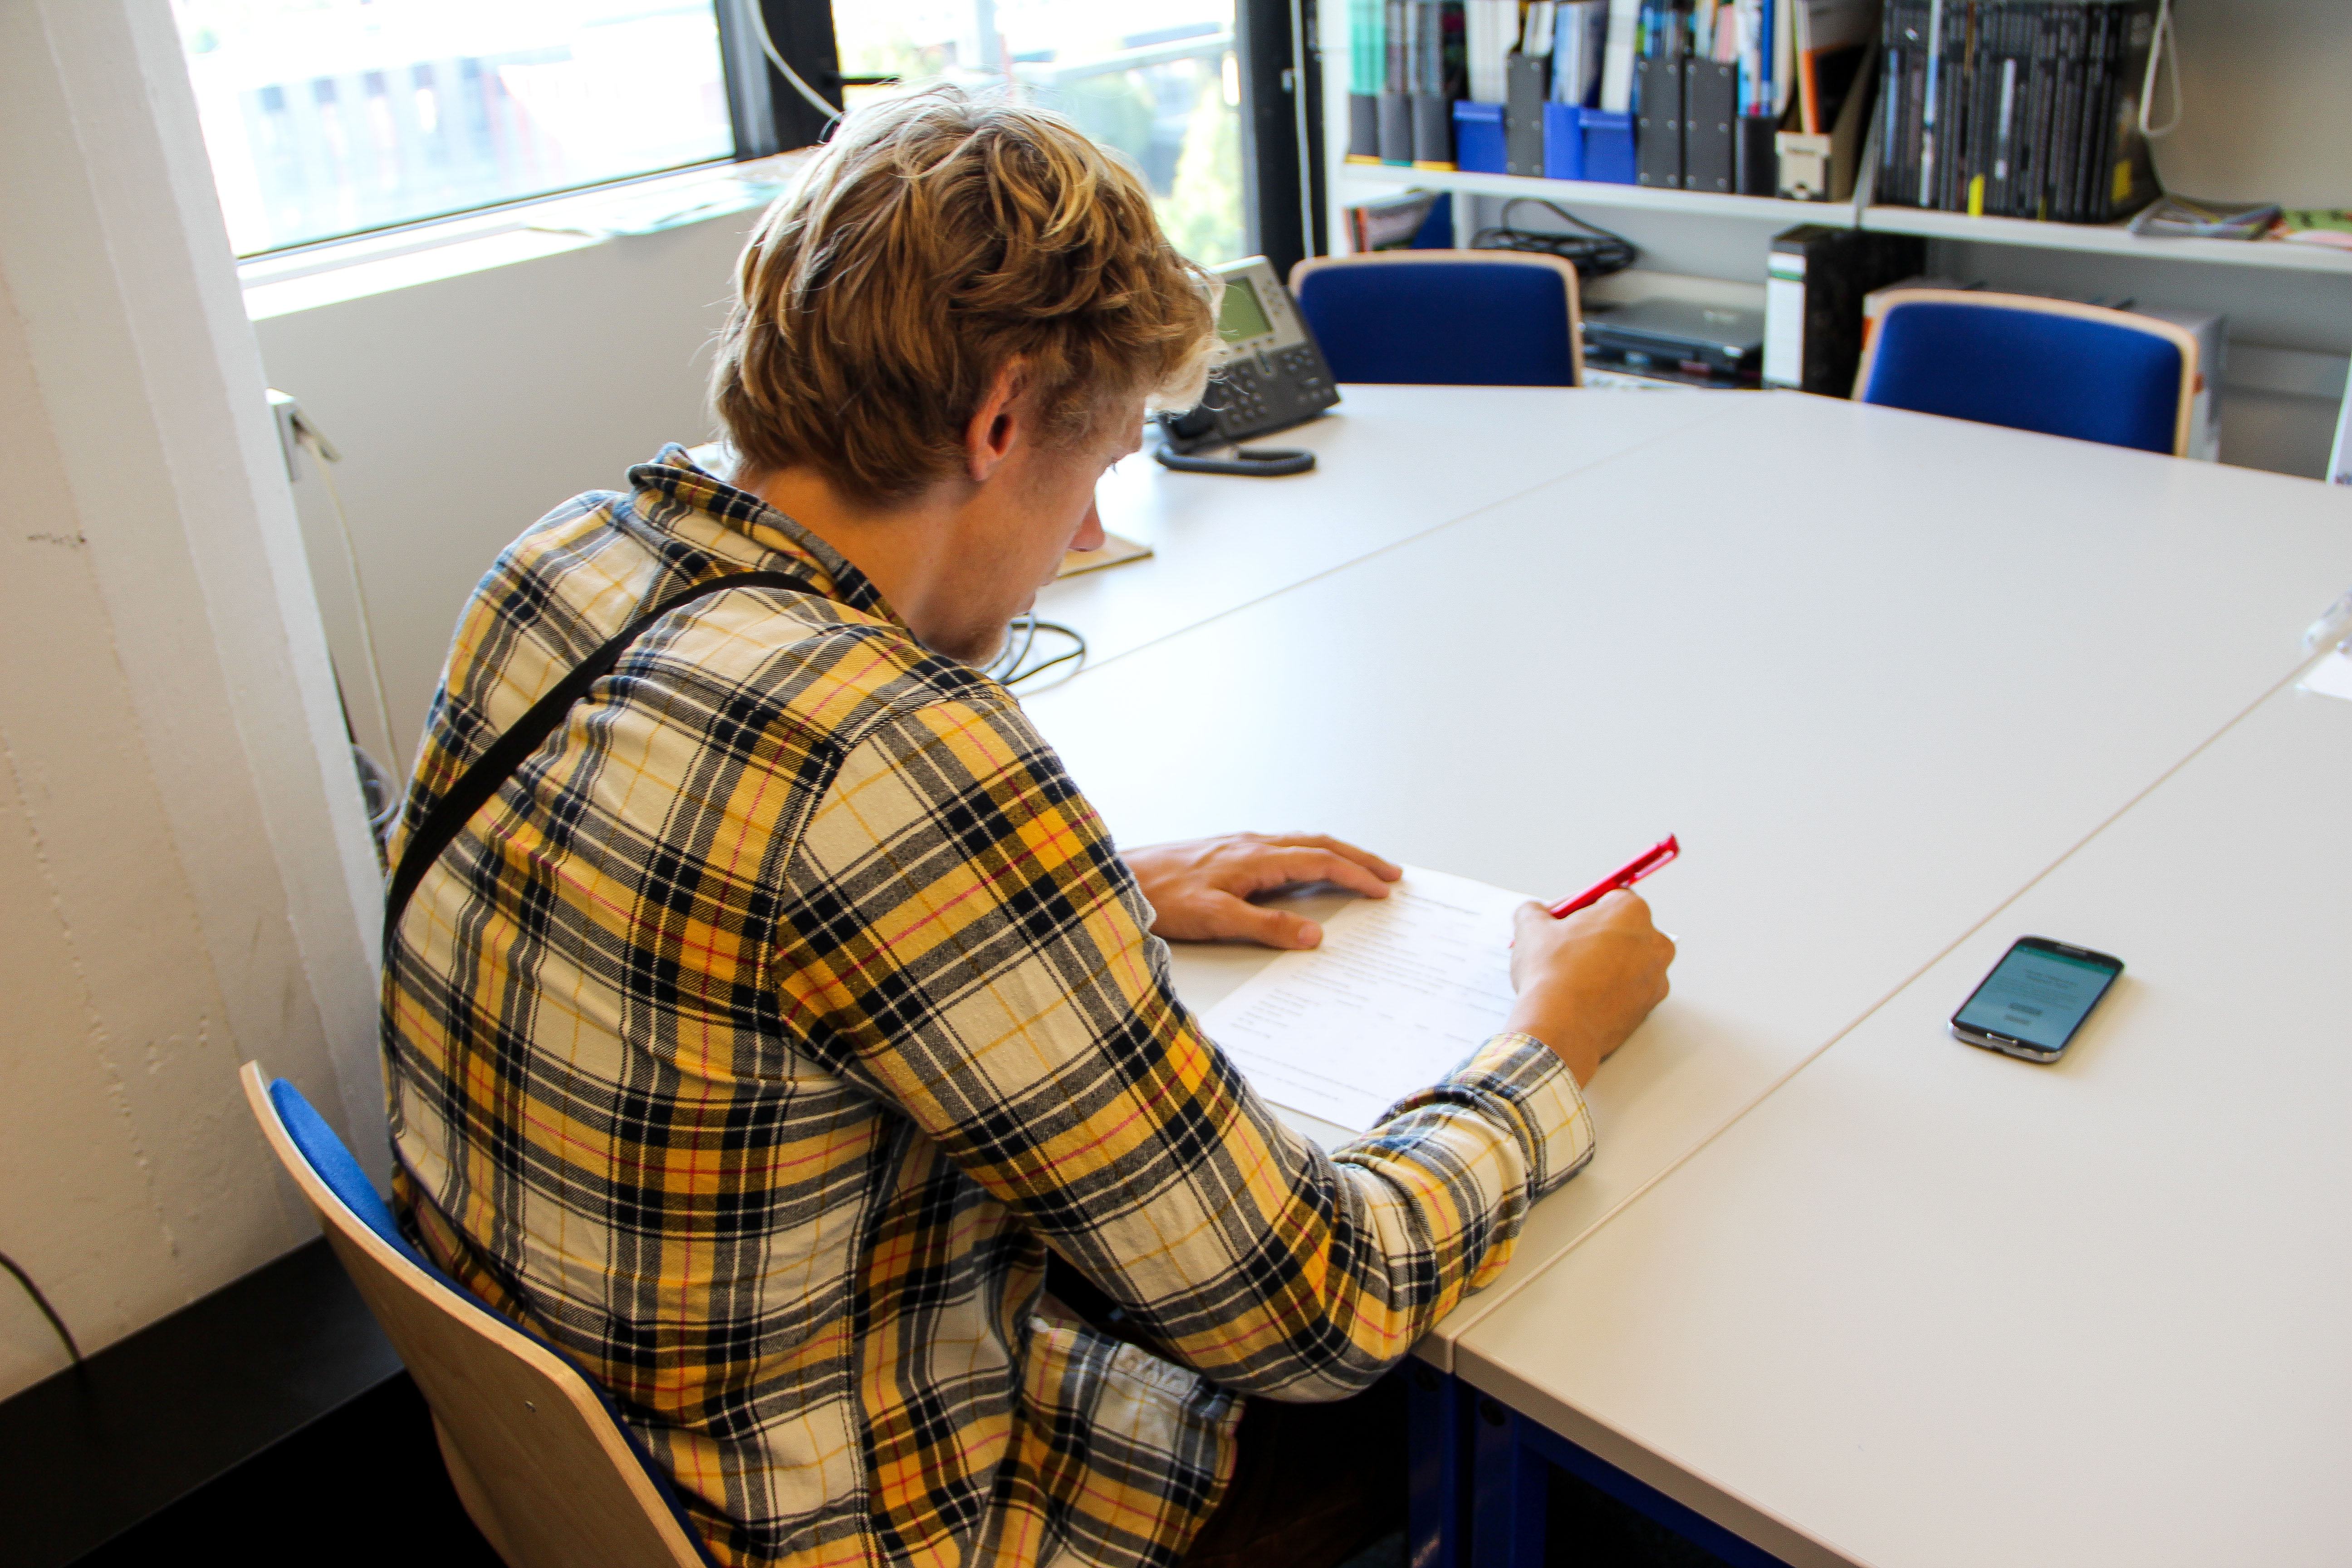
\includegraphics[width=0.67\textwidth]{img/prozedur3.jpg}}
\caption{Räumlichkeiten, Aufbau und Lichtverhältnisse während der Studie}
\label{prozedurumgebung}
\end{figure}
Die Studie findet innerhalb eines ruhigen und hellen Raumes statt, siehe Abbildung \ref{prozedurumgebung}. Der Testleiter sitzt rechts neben der Testperson an einem Tisch mit ausreichend Platz. Es soll hiermit sichergestellt werden, dass der Test von der Testperson ungestört und bei guten Lichtverhältnissen durchlaufen werden kann.

Jede Testperson hat ausschließlich freiwillig am Test teilzunehmen. Nach Betreten des Raumes erhält jede Testperson etwas zu trinken und wird zu ihrem Wohlbefinden befragt. Im Anschluss wird die Thematik sehr allgemein und knapp beschrieben. Danach wird der Testperson ein Studieninformationsblatt ausgehändigt, dass u.A. Anhaltspunkte über den allgemeinen Ablauf und die Datenverarbeitung enthält, siehe Anhang \ref{lab:Studieninformationen}.\\
Als nächstes wird ein Personenfragebogen der Testperson überreicht, die diesen direkt und mit ausreichend Zeit auszufüllen hat.\\
Damit die Testperson mit der Annäherungserkennung vertraut gemacht wird, stellt der Testleiter eine entsprechende Liste zur kurzen Demonstration vor. Die Testperson hat die Möglichkeit mit der Liste bei eingeschalteter Annäherungserkennung zu interagieren.

Anschließend wird die Testanwendung konfiguriert. Der Testleiter startet einen neuen Test mit der Angabe der korrekten Testgruppe und trägt dann die in der Testanwendung dargestellte Identifikationsnummer in die vorhergesehenen Felder auf den Fragebögen ein. Die Testumgebung wird nun der Testperson übergeben. Die Testperson wird gebeten, die Testbeschreibung durchzulesen und mögliche Fragen zu äußern. Sobald alle Fragen geklärt sind, beginnt die Testperson mit dem ersten Test.\\
Hat die Testperson den Test absolviert, wird ihr der System Usability Scale überreicht. Die Testperson hat diesen nun nach "`Bauchgefühl'" auszufüllen und kann im Anschluss mit der Wiederholung fortfahren.\\
Wurde auch für die zweite Testvariante der System Usability Scale ausgefüllt, leitet der Testleiter den zweiten Test ein. Die Testperson wird erneut gebeten, die Testbeschreibung durchzulesen und mögliche Fragen anzuzeigen. Danach kann die Testperson mit dem Test beginnen. Die Testanwendung ist so konfiguriert, dass in diesem Test von der Testperson bis zu 26 Schwierigkeitsgrade absolviert werden können. Die Schaltflächengröße wird mit jedem Schwierigkeitsgrad kontinuierlich verringert. Insgesamt wird der Test zwei Mal wiederholt und jede Testvariante ebenfalls mit einem System Usability Scale abgeschlossen.

Wurden alle Tests der Testanwendung vollständig absolviert, befragt der Testleiter die Testperson abschließend gemäß des qualitativen Fragebogens und notiert die gegebenen Antworten für die Testperson auf dem Fragebogen, um eine möglichst ausführliche Rückmeldung zu erhalten. 

\section{Design}\label{sec:design}
Die gesamte Testsitzung ist aufgeteilt in zwei Tests. Der erste Test besitzt einen Faktor mit zwei Levels und der zweite Test ist ein 3x26 Design. Beide Test sind within-subjects.

Der erste Test berücksichtigt die unabhängige Variable {\ttfamily Annäherungserkennung} mit den nominalen Zuständen {\ttfamily ausgeschaltet} und {\ttfamily eingeschaltet}. Der erste Test besitzt somit zwei Settings. Die abhängige Variable {\ttfamily Zeit} beschreibt die Zeitspanne (in ms) zwischen der Listeneinblendung bis zur richtigen Selektion der gesuchten Person. Bei Fehlselektionen wird die Variable nicht zurückgesetzt.

Der zweite Test berücksichtigt zwei unabhängige Variablen, {\ttfamily Schaltflächengröße} und {\ttfamily Annäherungserkennung}. Die unabhängige Variable {\ttfamily Schaltflächengröße} besitzt 26 rationale Zustände, beginnend bei \emph{10mm} und endend bei \emph{1.4mm}. Die unabhängige Variable {\ttfamily Annäherungserkennung} besitzt die nominalen Zustände \emph{ausgeschaltet}, \emph{eingeschaltet} und \emph{eingeschaltet mit Selektionshilfe}. Der Test ermittelt für jedes Setting die Werte von vier abhängigen Variablen: Die {\ttfamily Gesamtzeit} (in ms) gibt die Zeitspanne zwischen der Fingeranhebung nach der ersten Blaufärbung der Zielschaltfläche bis zur Berührung dieser Schaltfläche an - bei Fehlberührungen wird die Variable nicht zurückgesetzt. Die abhängige Variable {\ttfamily Zeit} wird dabei vor jedem Neuversuch zurückgesetzt. Die {\ttfamily Fehlerzahl} gibt die Anzahl der Fehlberührungen an. Diese Variable wird den Wert \emph{5} nicht übersteigen, da nach dem vierten Fehlversuch der Test vorzeitig beendet und der Wert auf \emph{5} erhöht wird. Bei einem Testabbruch wird zusätzlich die abhängige Variable {\ttfamily Abbrüche} von \emph{0} auf \emph{1} gesetzt.\\
Sollten einige Settings aufgrund eines Testabbruchs übersprungen worden sein, so bleiben für diese Settings die abhängigen Variablen {\ttfamily Zeit} und {\ttfamily Gesamtzeit} in der Auswertung unberücksichtigt. Die abhängige Variable {\ttfamily Fehlerzahl} wird in diesem Fall auf den Wert \emph{5} und die abhängige Variable {\ttfamily Abbrüche} auf den Wert \emph{1} gesetzt.

Um ein Counterbalancing zu erwirken, wurden gemäß des Latin Squares die Tests in mehrere Reihenfolgen durchlaufen. Der erste Test benötigt gemäß der Zustandsanzahl der unabhängigen Variable {\ttfamily Annäherungserkennung} zwei Reihenfolgen. Der zweite Test muss für ein entsprechendes Counterbalancing aufgrund des zusätzlichen Zustands \emph{eingeschaltet mit Selektionshilfe} mit drei verschiedenen Reihenfolgen getestet werden.

\chapter{Ergebnisse}
In diesem Kapitel wird die Auswertung der erhobenen Daten erläutert und die Ergebnisse der Studie präsentiert.

Die Protokolldaten wurden anhand eines eigens entwickelten Programms analysiert und für die statistische Auswertung unter R aufbereitet. Die Protokolldaten, das entsprechende Programm und die aufbereiten Daten sind in digitaler Form auf dem beiliegenden Datenträger dieser Bachelorarbeit gespeichert. Darüber hinaus finden sich auch die Quelltexte für R inklusive aller grafischen Datendiagramme auf diesem Datenträger.

Bevor es jedoch zu einer statistischen Auswertung kam, wurden alle fehlerhaften Werte mit deutlichen Messfehlern entfernt. Im zweiten Test verkleinerte sich dadurch die Gesamtzahl der Trials von 1404 auf 1402. Im ersten Test fand innerhalb der 252 Trials keine Verringerung statt. 

\section{Test 1: Listenauswahl}
\begin{figure}
\centering
\includegraphics[width=0.68\textwidth]{img/BoxplotTest1.png}
\caption{Kastengrafik mit den Zeitwerten für beide Settings aus Test 1.}
\label{ergebnistest1}
\end{figure}
Die durchschnittliche Gesamtzeit über alle Trials beträgt $7305.7$ ms. Trennt man die Gesamtzeiten in die beiden Settings auf, so lag die durchschnittliche Gesamtzeit mit eingeschalteter Annäherungserkennung bei $7290.7$ ms und ist damit um $0.41\%$ kleiner als mit ausgeschalteter Annäherungserkennung mit $7320.8$ ms. Zur Übersicht stellt die Abbildung \ref{ergebnistest1} die Ergebnisse der beiden Settings grafisch dar.\\
Die Unterschiede zwischen den Gesamtzeiten der beiden Settings waren nicht signifikant ($F_{1,6}\approx 0.003, p > .05$).\\
Ein signifikanter Unterschied bestand jedoch zwischen den zu suchenden Personeneigenschaften ($F_{6,6}\approx 8.558, p < .05$). Ein etwaiger Einfluss der Personeneigenschaften auf die Gesamtzeiten zwischen den beiden Settings ist damit nicht auszuschließen.

\section{Test 2: Präzisionstest}
Zur Auswertung des zweiten Tests wurden die verbliebenen Testpersonen für jede Schaltflächengröße anhand der Anzahl der Abbrüche ermittelt und grafisch in einem Balkendiagramm dargestellt, siehe Abbildung \ref{ergebnistest2survivals:10mm}.\\
Das Diagramm zeigt, dass sich die Anzahl der verbliebenen Testpersonen bis zu einer Schaltflächengröße von $4.5$ mm nicht verringerte. Bei Schaltflächengrößen von mindestens $2.8$ mm verblieben die Testpersonen mit ausgeschalteter Annäherungserkennung mindestens genauso lange im Test, während sich die Anzahl der Testpersonen mit aktiverer Selektionshilfe leicht verringerte. Bei Schaltflächengrößen zwischen $2.4$ mm und $1.4$ mm verblieben jedoch mehr Testpersonen mit Annäherungserkennung oder Selektionshilfe im Test.\\
\begin{figure}
\centering
\subfigure[Schaltflächengrößen von $10$ mm bis $1.4$ mm]{\includegraphics[width=\textwidth]{img/BarplotTest2Survivals.png}\label{ergebnistest2survivals:10mm}}
\subfigure[Schaltflächengrößen von $2.4$ mm bis $1.4$ mm]{\includegraphics[width=\textwidth]{img/BarplotTest2SurvivalsSubset.png}\label{ergebnistest2survivals:2.4mm}}
\caption{Balkendiagramm der verbliebenen Testpersonen aus Test 2.}
\label{ergebnistest2survivals}
\end{figure}
Betrachtet man den Test mit allen Schaltflächengrößen von $10$ mm und $1.4$ mm, so wurden keine signifikanten Unterschiede zwischen der Anzahl der verbliebenen Testpersonen in den jeweiligen Settings festgestellt ($F_{2,17}\approx 1.831, p > .05$). Signifikante Unterschiede sind festzustellen, sobald der Test ausschließlich mit den Schaltflächengrößen von $2.4$ mm bis $1.4$ mm betrachtet wird ($F_{2,3}\approx 8.725, p < .05$). Die Abbildung \ref{ergebnistest2survivals:2.4mm} stellt diesen Wertebereich übersichtlich in einer Vergrößerung dar. Die signifikanten Unterschiede wurden mittels eines t-Test für gepaarte Stichproben ermittelt. Die Anzahl der verbliebenen Testpersonen ist in den Settings mit ausgeschalteter Annäherungserkennung ($M = 9.75, SD\approx 4.03$) signifikant kleiner als in den Settings mit eingeschalteter Annäherungserkennung ($M = 14.5, SD\approx 2.52, t(???) =??? , p < .05$) bzw. mit aktivierter Selektionshilfe ($M = 14.75, SD = 0.50, t(???) = ??? , p < .05$).

Um die Geschwindigkeit jedes Settings zu bewerten, wurden die Parameter aus den Rohdaten in ein Modell nach Fitt's Law transferiert. Hierzu wurden zunächst die unrealistisch kleinen Zeiten und die oberen Ausreißer entfernt ($p = 0.75$). Für jede Testperson wurde anschließend ein Diagramm erstellt, dass für jede Schaltflächengröße und Annäherungserkennung den "`Index of Difficulty"' und die Zeit (siehe Abschnitt~\ref{sec:design}) in einem Koordinatensystem darstellt. Im darauffolgenden Schritt wurde pro Annäherungserkennung eine Regressionsgerade über die Punkte inklusive dem dazugehörigen Korrelationskoeffizienten berechnet. Die Abbildung \ref{ergebnistest2fitts} zeigt den Datensatz einer Testperson.
\begin{figure}
\centering
\includegraphics[width=0.68\textwidth]{img/fittsUser12.png}
\caption{Diagramm zur Bewertung von Fitt's Law.}
\label{ergebnistest2fitts}
\end{figure}
Nach einer anfänglichen Begutachtung der Diagramme aller Testpersonen und einer darauffolgenden statistischen Auswertung wurde deutlich, dass sich die Steigungen der Regressionsgerade je Annäherungserkennung immer signifikant voneinander unterscheiden ($F_{2,17}\approx 13.063, p < .05$). Mittels eines t-Test für gepaarte Stichproben wurden die signifikanten Unterschiede für jedes Settings-Paar ermittelt. Die Steigung der Regressionsgerade für die Trials mit Selektionshilfe war dabei am steilsten ($M = 284.10, SD \approx 177.44$) und damit, sowohl signifikant größer ($t(???) =??? , p < .05$) gegenüber der Steigung mit eingeschalteter Annäherungserkennung ($M \approx 81.93, SD \approx 142.27$) als auch signifikant größer ($t(???) =??? , p < .05$) gegenüber der Steigung mit ausgeschalteter Annäherungserkennung ($M = 77.04, SD \approx 46.68$). Auch die Steigung mit ausgeschalteter Annäherungserkennung war gegenüber der Steigung mit eingeschalteter Annäherungserkennung signifikant kleiner ($t(???) =??? , p < .05$).

\section{System Usability Scale}
\begin{figure}
\centering
\subfigure[Test 1: Listenauswahl]{\includegraphics[width=0.49\textwidth]{img/BoxplotSUSTest1.png}}
\hfill
\subfigure[Test 2: Präzisionstest]{\includegraphics[width=0.49\textwidth]{img/BoxplotSUSTest2.png}}
\caption{Kastengrafik mit den Scores des System Usability Scales für die Testreihen in beiden Tests.}
\label{ergebnisSUS}
\end{figure}
Nach der Auswertung aller System Usability Scales, siehe Abbildung \ref{ergebnisSUS}, wurde für den ersten Test ein durchschnittlicher Score von $81.8$ ermittelt. Nach Auftrennung der Scores in die beiden Settings, lag der durchschnittliche Score mit eingeschalteter Annäherungserkennung bei $80.6$ und ist damit kleiner als mit ausgeschalteter Annäherungserkennung mit $83.1$.\\
Der zweite Test erhielt einen durchschnittlichen Score von $74.3$. Durch die Auftrennung der Scores in die drei Settings, erhielt das Setting mit eingeschalteter Annäherungserkennung bei einem durchschnittliche Score von $75.8$ den höchsten Wert. Das Setting mit ausgeschalteter Annäherungserkennung erhielt mit einem durchschnittlichen Score von $73.6$ den zweithöchsten Wert. Das Setting mit aktivierter Selektionshilfe erhielt bei einem durchschnittlichen Score von $73.3$ den kleinsten Wert.\\
Nach der statistischen Betrachtung wurden sowohl für den ersten Test ($F_{1,17}\approx 0.246, p > .05$) als auch für den zweiten Test ($F_{2,17}\approx 1.937, p > .05$) keine signifikanten Unterschiede zwischen den Settings festgestellt. In beiden Tests fielen die Scores je Annäherungserkennung jedoch überdurchschnittlich aus \citep{sus2013}.

Noch was dazu sagen, warum man die anderen dinge nicht ausgewertet hat (MISTAKES ETC)?

\chapter{Diskussion}
Die statistischen Ergebnisse des ersten Tests deuten nicht darauf hin, dass durch die Annäherungserkennung eine Verbesserung der Usability während der Interaktion mit Listen erwirkt wird. Auch die Ergebnisse des System Usability Scores zeigen, dass sich die Usability bei eingeschalteter Annäherungserkennung verschlechterte.\\
Das schlechte Abschneiden des ersten Tests ist höchstwahrscheinlich auch durch den Testaufbau stark beeinflusst worden: Durch die Notizen des Testleiters wurde festgestellt, dass 5 von 18 Personen die Hervorhebungen mangels fehlender Fingerannäherung nicht gesehen haben. Zudem gaben 9 von 18 Testpersonen explizit an, dass ihnen der Testaufbau nicht gefallen hat: Entweder hielten sie die Listeneinträge aufgrund der Hervorhebungen bei Annäherung für Schaltflächen oder sie bemängelten die Bedienung in zwei Schritten. Dementsprechend wäre das direkte Anwählen der Listen intuitiver gewesen, anstatt zusätzliche Schaltflächen am unteren Bildschirmrand zu verwenden.\\
Aus diesem Grund wäre ein erneuter Testdurchgang mit anwählbaren Schaltflächen interessant. Die Hervorhebungen bei Annäherung können nämlich bei richtiger Umsetzung für die Nutzer durchaus eine Hilfestellung sein. Immerhin haben 7 von 18 Testpersonen angegeben, dass ihnen die Hervorhebungen im ersten Test als hilfreich in Erinnerung geblieben sind. Zudem sind im Bezug auf die Schaltflächenidentifizierung die Beobachtungen des Testleiters interessant: Bei mehreren Testpersonen wurde beobachtet, dass diese die Listeneinträge während der Hervorhebungen bei der Annäherung anschließend anwählten und sie somit von der Testbeschreibung abwichen.

Die Bewertung bei eingeschalteter Annäherungserkennung viel im zweiten Tests hingegen deutlich besser aus. So gaben im qualitativen Fragebogen 14 von 18 Personen an, dass die Hervorhebungen bei der Lösung der Aufgaben geholfen haben. Die Ergebnisse des System Usability Scores bestätigen diese Annahme, da sich diese bei eingeschalteter Annäherungserkennung im Vergleich zu den beiden anderen Alternativen leicht verbessern. Betrachtet man die statistischen Ergebnisse zur verbliebenen Nutzeranzahl pro Schaltflächengröße, zeigt sich, dass die eingeschaltete Annäherungserkennung bei sehr kleinen Schaltflächen ab $2.4$ mm signifikant besser abschneidet und die Nutzer bei derartigen Szenarios unterstützt. Dies würde beispielsweise eine Implementation der Annäherungserkennung in Anwendungen rechtfertigen, die über sehr kleine Schaltflächen verfügen, u.A. in Kartenanwendungen oder im Internetbrowser bei kleinen Zoomstufen.\\
Bei größeren Schaltflächen konnten keine signifikanten Unterschiede festgestellt werden. Ob die Annäherungserkennung auch in diesen Fällen eingeschaltet werden sollte, ist möglicherweise eine nutzerspezifische Frage: Im qualitativen Fragebogen gaben nämlich 6 von 18 Testpersonen an, dass die Hervorhebungen gelegentlich unpräzise und störend waren. Zudem ist laut den Ergebnissen zu Fitt's Law erkennbar, dass sich die Zeitdauer bis zur endgültigen Ausführung einer Interaktion mit eingeschalteter Annäherungserkennung erhöhte.

Die Selektionshilfe erhielt für den System Usability Score die, wenn auch geringfügig, schlechtesten Ergebnisse. Die Zeitdauer bis zur endgültigen Ausführung einer Interaktion war bei der Selektionshilfe laut der Auswertung nach Fitt's Law ebenfalls am höchsten. Bei Schaltflächen in einem Größenbereich von $2.4$ mm bis $1.4$ mm ist die Implementation einer Selektionshilfe dennoch denkbar, da die Anzahl der verbliebenen Nutzer mit dieser Methode am höchsten war. Natürlich ist eine Anpassung des Algorithmus nötig, um die Präzision und Geschwindigkeit der Selektionshilfe weiter zu optimieren.

\section{Vergleich zu den bisherigen Leitfäden}
Die Erkenntnisse, die innerhalb dieser Bachelorarbeit erlangt wurden, deuten darauf hin, dass eine Verringerung der Mindestgrößen für Bedienelemente trotz Annäherungserkennung nicht sinnvoll wären. Zwar konnte die Präzision der Touchposition bei Schaltflächengrößen zwischen $2.4$ mm und $1.4$ mm durch Einblenden von Hervorhebungen bei Fingerannäherung erhöht werden, jedoch erfolgt dies in einem sehr kleinen, von $7$ mm weit entferntem, Größenbereich und eine Implementation ist somit nur in derartigen Spezialfällen ratsam. Darüber hinaus bleibt das Fat-Finger-Problem ungelöst: Im qualitativen Fragebogen gaben 7 von 18 Testpersonen an, dass sie diesen Umstand als störend empfanden.\\
Hinzu kommt die mangelnde Unterstürzung dieser Technologie seitens der Hardwarehersteller, sowie die noch zu geringe Geschwindigkeit und Genauigkeit der Fingerlokalisierung auf mobilen Endgeräte mit bereits integrierter Annäherungserkennung.

\section{Limitierungen}
Trotz aller Bemühungen die Tests bestmöglich auszuführen, hat durch das universitäre Umfeld eine indirekte Fokussierung der Testpersonen stattgefunden. Gerne hätte ich auch ältere Personen in meiner Studie die Testanwendung testen lassen. Allerdings haben sich hauptsächlich junge Menschen gemeldet. Auch eine Akquise meinerseits änderte daran nichts. Die wenigen in Frage gekommenen Testpersonen mit hohem Alter (z.B. Seniorenalter) konnten somit leider nicht teilnehmen, da dem Schaffen einer möglichst homogenen Gruppe eine höhere Priorität eingeräumt wurde.

Auch der Umfang der Tests hätte durchaus ausgeweitet werden können. Zwar wurden auch die genannten Parameter zur Bestimmung der Fehlerrate und Ausführungszeit protokolliert und statistisch untersucht, jedoch hätte eine wissenschaftliche Auswertung mit hinreichender Güte den Umfang dieser Bachelorarbeit weit überstiegen.

\chapter{Fazit}
Im Rahmen dieser Bachelorarbeit wurde für ein verbessertes Verständnis der Usability von Annäherungserkennung und zur Überprüfung der Mindestgrößen von Bedienelementen eine Studie durchgeführt. Hierzu wurde vom Studenten eine eigens entwickelte Testanwendung konzipiert und implementiert. Nachdem die 18 Testpersonen die Tests innerhalb der Testanwendung mehrmals wiederholten, wurden durch statistische Analysen der erhobenen Daten die Unterschiede mehrerer Parameter unter Berücksichtigung der jeweiligen Zustände der Annäherungserkennung ermittelt.

Auch wenn die Ergebnisse der System Usability Scores für die jeweiligen Annäherungserkennungen sich in beiden Tests nicht signifikant voneinander unterscheiden, konnten die qualitative Fragebögen zeigen, dass die Annäherungserkennung von der Mehrheit der Nutzer angenommen und bevorzugt wird. Nach dem subjektiven Empfinden der Nutzer unterstützte es sie bei der Erledigung ihrer Aufgaben.

Bei Tests mit Listeneinträgen konnte kein signifikanter Unterschied zwischen den Bearbeitungszeiten bei ein- und ausgeschalteter Annäherungserkennung gefunden werden. Beim Präzisionstest unterschied sich bei üblichen Schaltflächengrößen die Anzahl der verblieben Testpersonen im Test kaum. Lediglich bei Schaltflächengrößen zwischen $2.4$ mm und $1.4$ mm konnten, wie auch während der aktivierten Selektionshilfe, signifikant mehr Testpersonen im Test verbleiben. Laut den Ergebnissen zu Fitt's Law erhöhte sich mit eingeschalteter Annäherungserkennung die Zeitdauer bis zur endgültigen Ausführung einer Interaktion. Die Zeitdauer war zum Vergleich bei ausgeschalteter Annäherungserkennung am geringsten und während der aktivierten Selektionshilfe am größten. Dabei waren die Unterschiede jeder Zeitdauer bei allen Kombinationen signifikant unterschiedlich.

Als Ausblick wäre für die weitere Forschung eine Auswertung der verbleibenden Datensätze interessant. Die gesamten Daten befinden sich ebenfalls auf dem beiliegendem Datenträger. Das größte Potential ergibt sich meiner Meinung nach bei der Optimierung der Selektionshilfe, die zu einem fortgeschrittenem Forschungsstand idealerweise die Touchpositionen des Nutzers unbemerkt im Hintergrund optimiert. Es wäre denkbar, dass sich somit besonders kleine Schaltflächen mit wenig Aufwand anwählen lassen. Mögliche Einsatzgebiete für eine derartige Selektionshilfe ergeben sich beispielsweise in Kartenanwendungen und Webseiten bei geringen Zoomstufen, auf Bedienoberflächen für Platzreservierungen und bei Bildschirmtastaturen.

Weitere mögliche Forschungsgebiete bestehen in Szenarien der Textselektion und Schaltflächenidentifizierung, z.B. durch visuelle Hervorhebungen bei Annäherung.\\
Alternativ wären anstatt von Hervorhebungen zusätzliche visuelle Ebenen denkbar, z.B. die Entwicklung eines Fingerpositionszeigers mit einem beliebigen Positionsversatz zur Lösung des Fat-Finger-Problems. Eine anfängliche Implementation findet sich ebenfalls im Quelltext der Testanwendung. Der Quelltext ist auf dem beiliegendem Datenträger gespeichert.

Unabhängig von den oberen Themen, ließe sich auch im Hardwarebereich forschen. So könnte die Annäherungserkennung in diesem Feld von Geschwindigkeits- und Genauigkeitserhöhungen bei der Fingerlokalisierung profitieren. Eventuell lassen sich auch geeignete Szenarien für die Annäherungserkennung finden, bei denen die Nutzung von mehreren Fingern einen mit einem Mehrwert verbunden sind. In diesem Fall müssen auch hardwareseitig die nötigen Voraussetzung geschaffen werden.

\begin{appendix} 
\chapter{Anhang}
\newpage
\section{Studieninformationen}
\frame{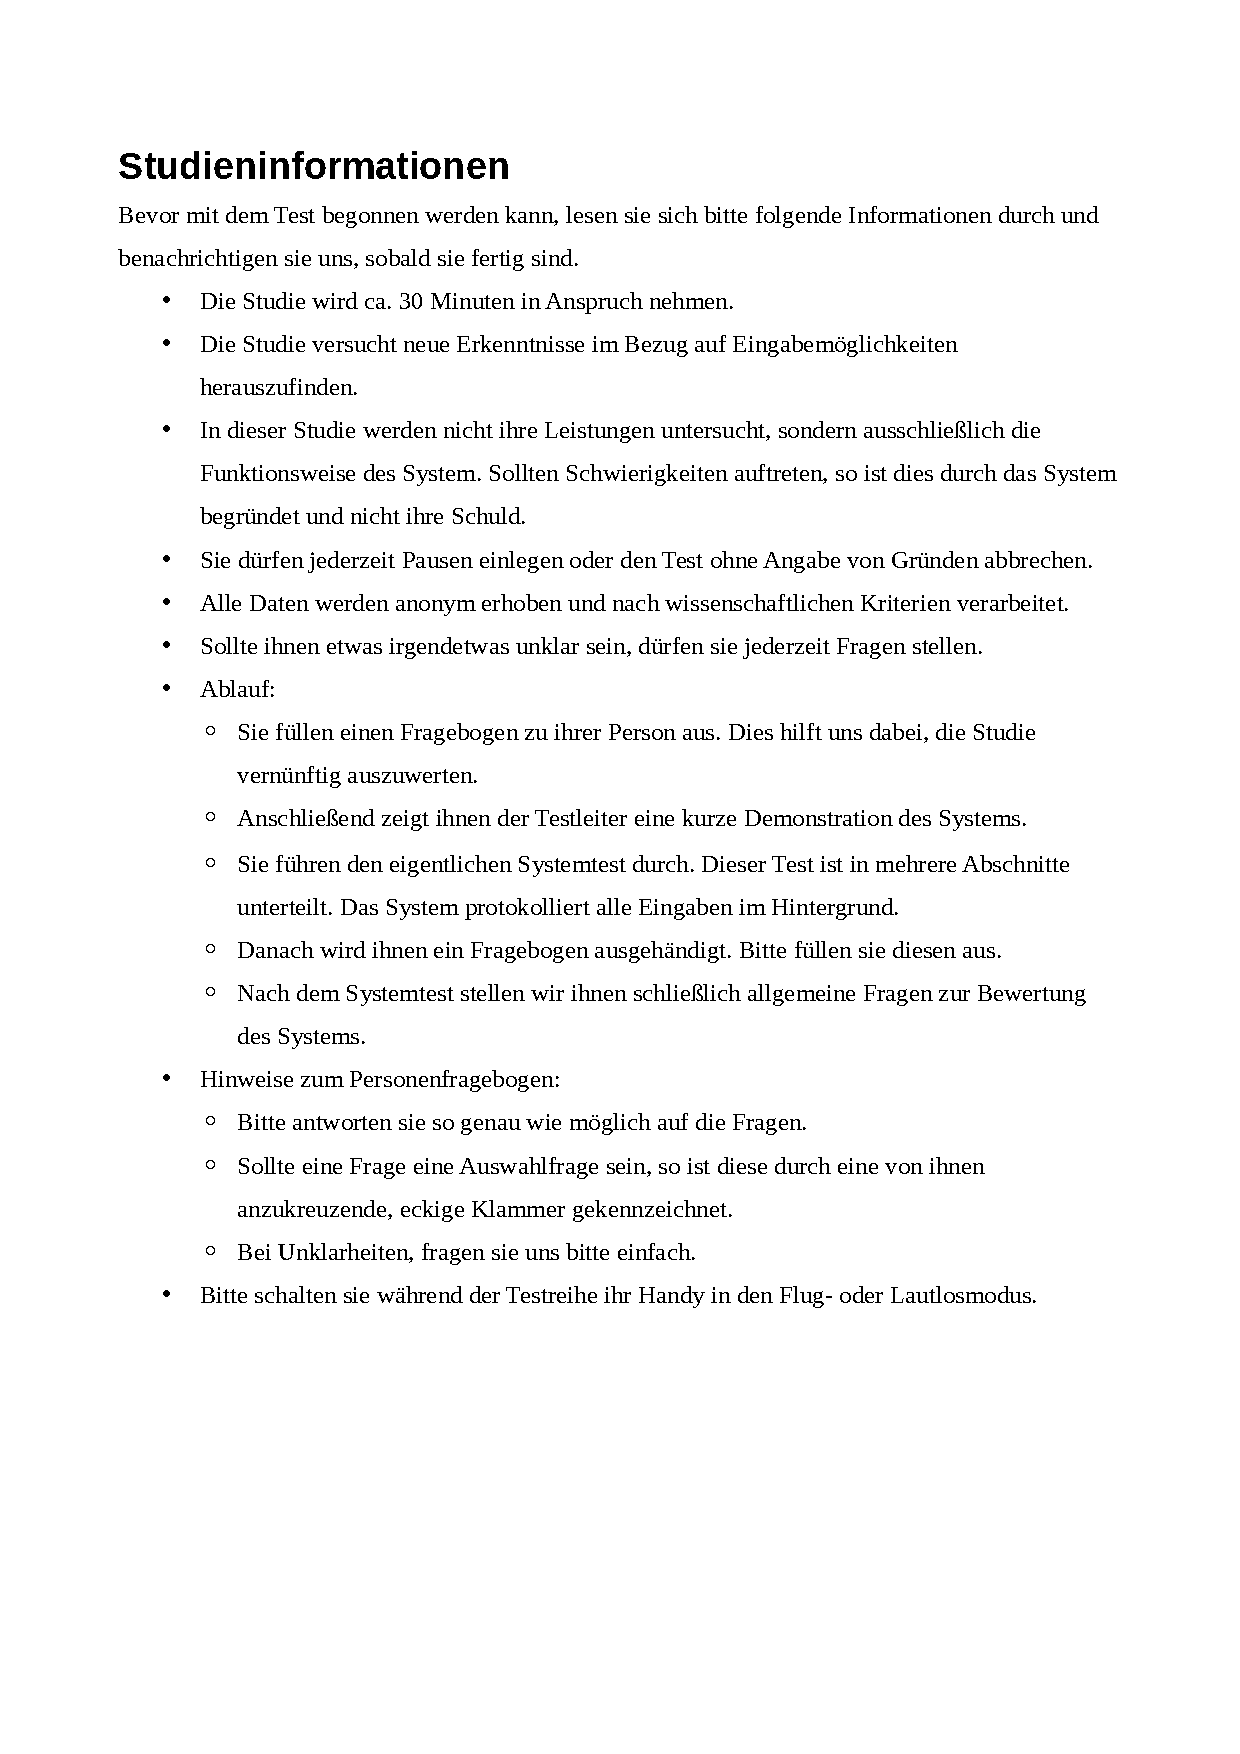
\includegraphics[width=\textwidth, page=1]{apx/Studieninformationen}}
\label{lab:Studieninformationen}

\section{Personenfragebogen}
\frame{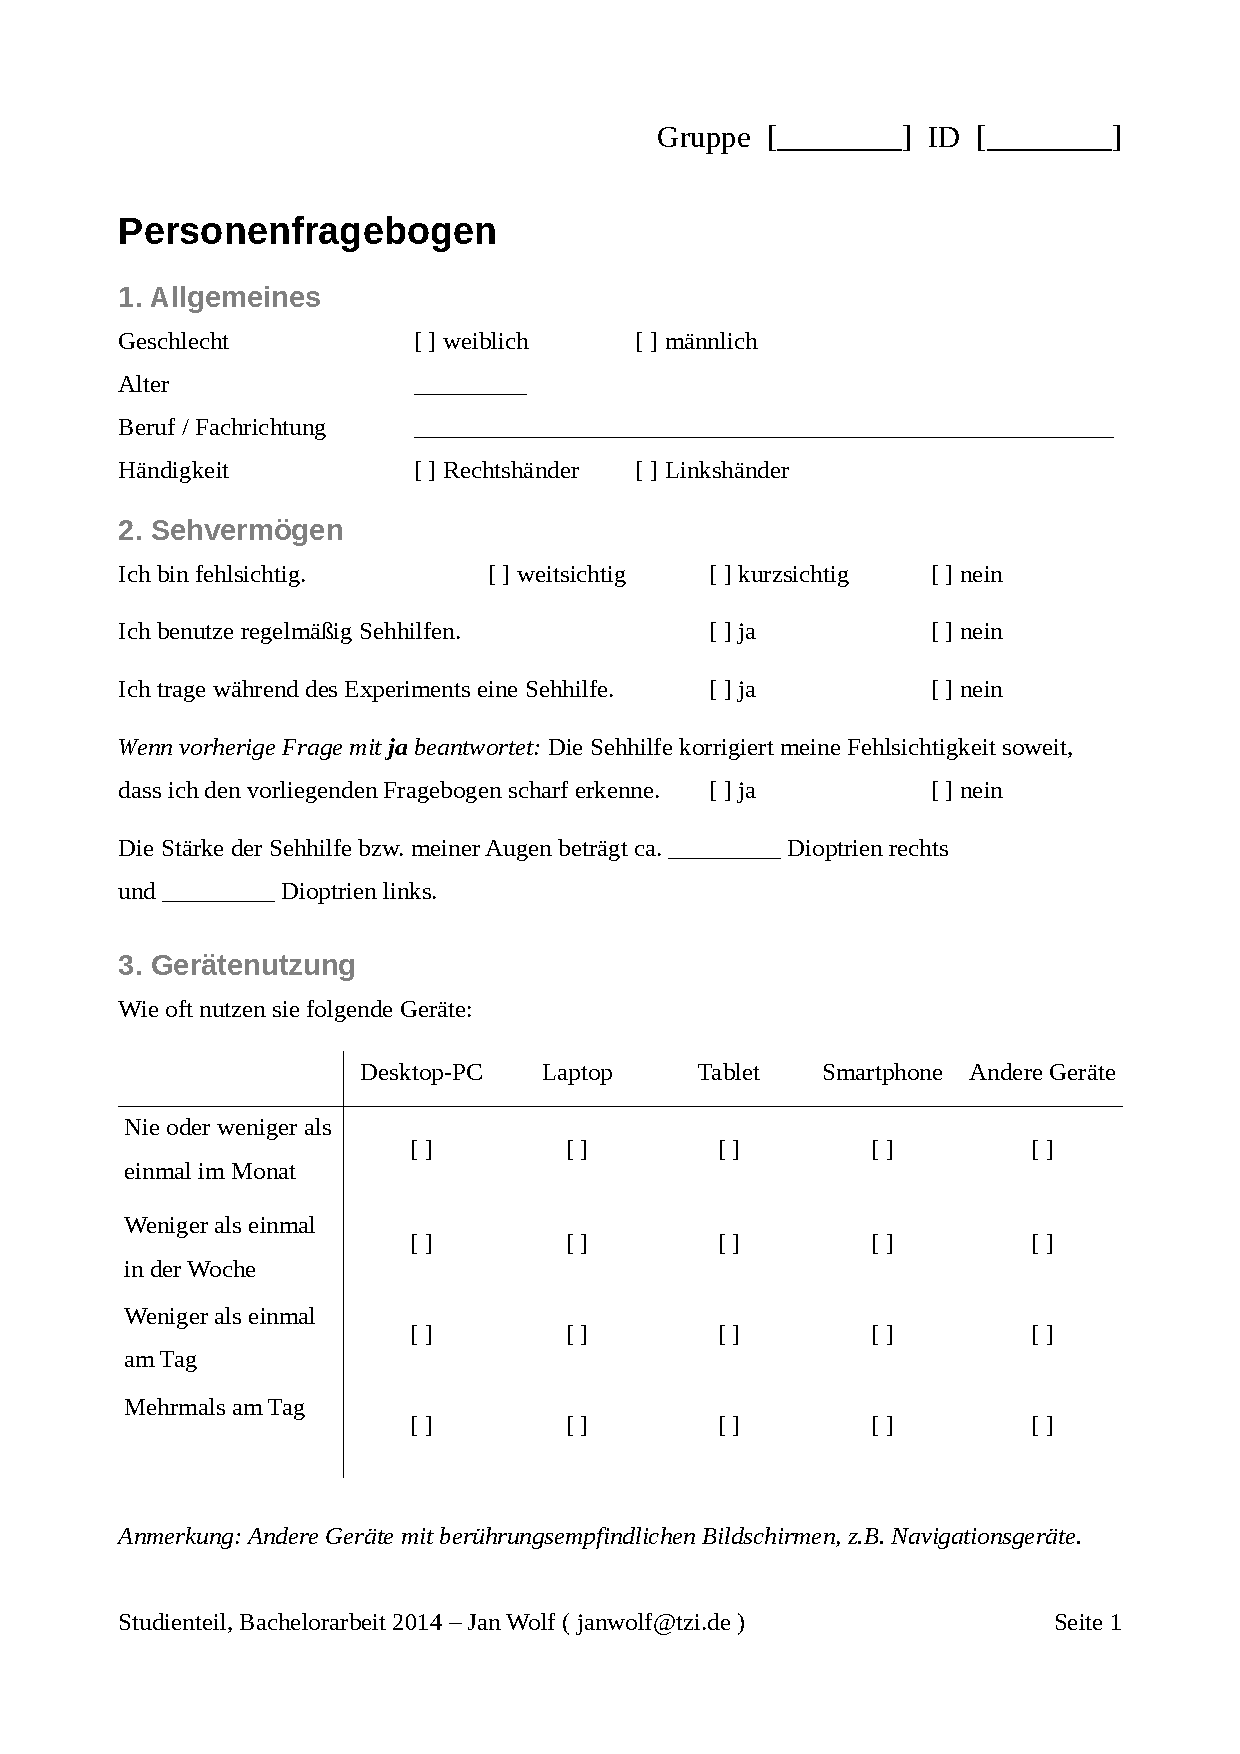
\includegraphics[width=\textwidth, page=1]{apx/Personenfragebogen}}
\label{lab:Personenfragebogen}

\frame{\includegraphics[width=\textwidth, page=2]{apx/Personenfragebogen}}
 
\section{Bewertungsbögen}
\frame{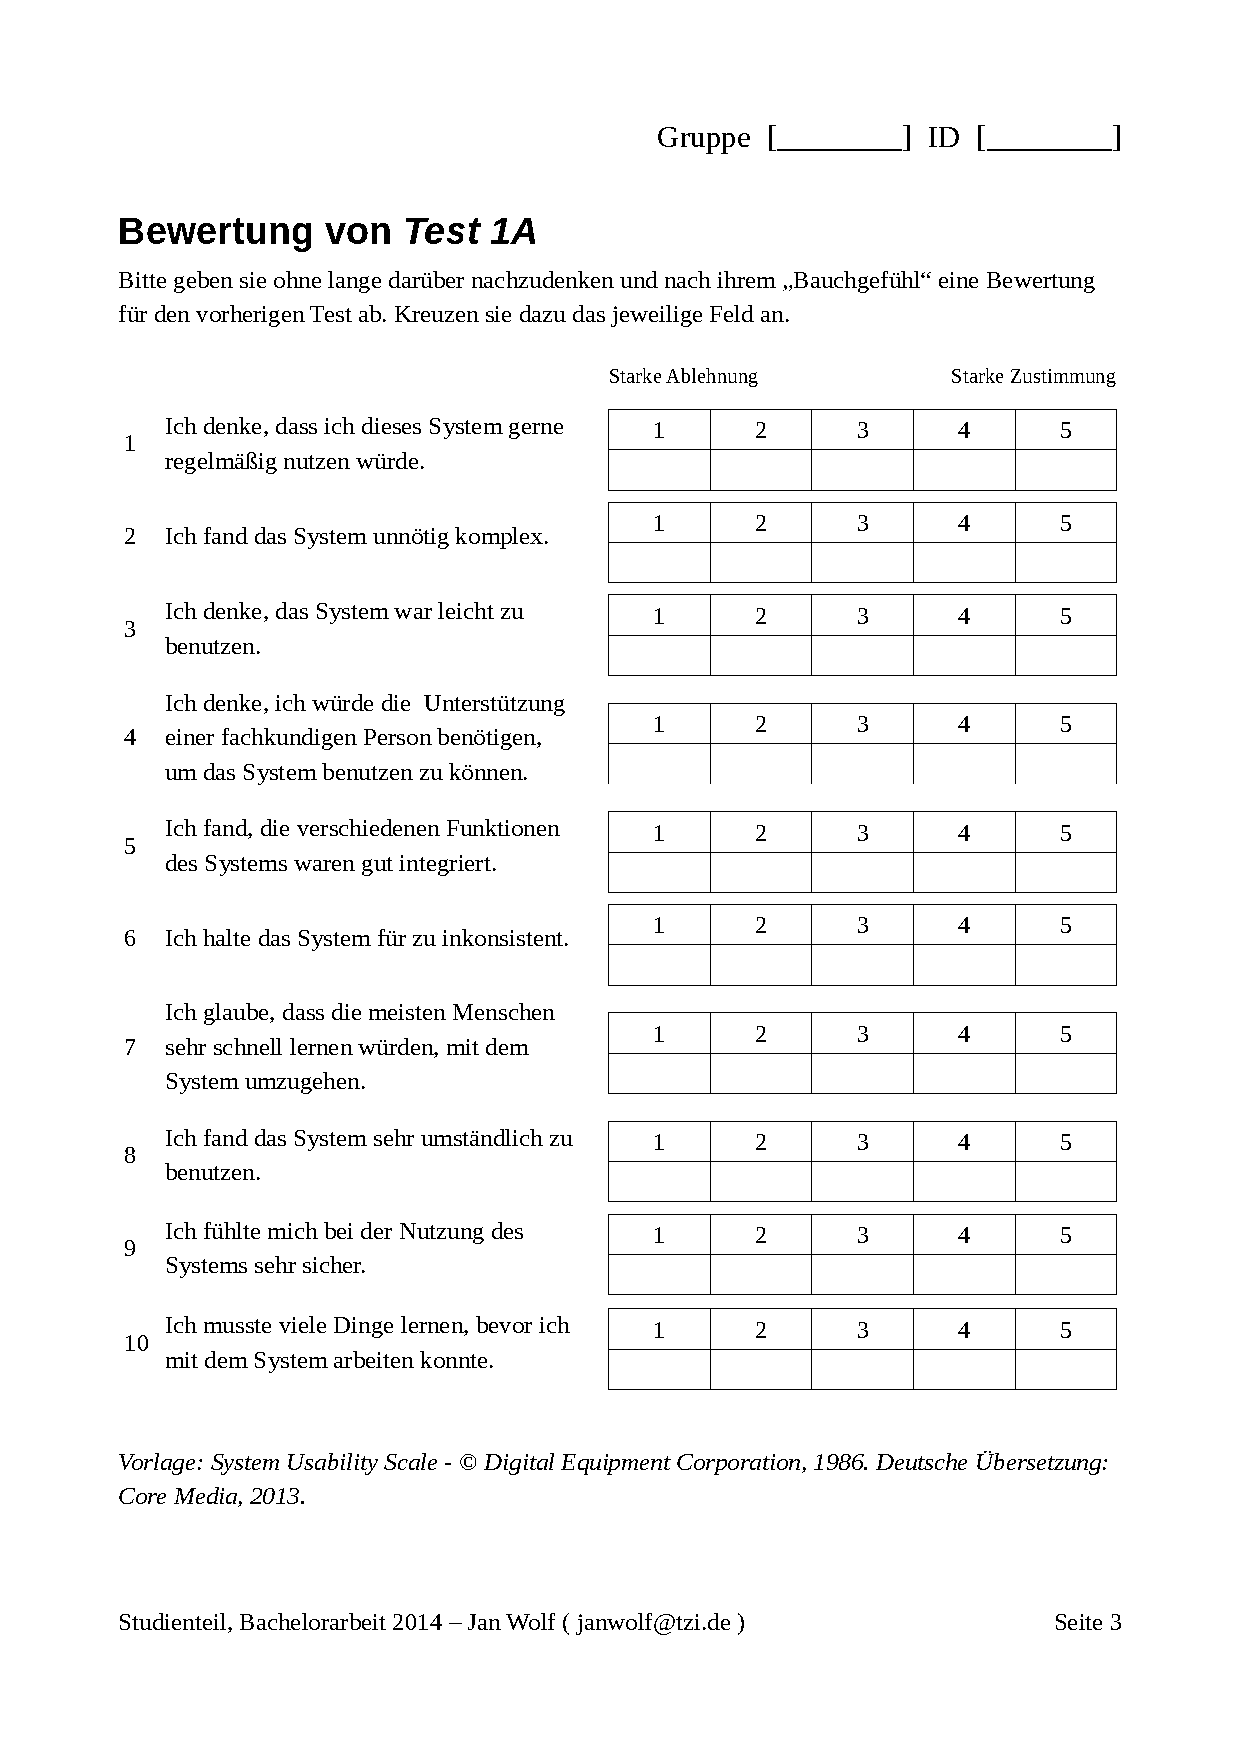
\includegraphics[width=\textwidth, page=1]{apx/Bewertungsboegen}}
\label{lab:Bewertungsbögen}

\frame{\includegraphics[width=\textwidth, page=2]{apx/Bewertungsboegen}}

\frame{\includegraphics[width=\textwidth, page=3]{apx/Bewertungsboegen}}

\frame{\includegraphics[width=\textwidth, page=4]{apx/Bewertungsboegen}}

\frame{\includegraphics[width=\textwidth, page=5]{apx/Bewertungsboegen}}

\frame{\includegraphics[width=\textwidth, page=6]{apx/Bewertungsboegen}}

\end{appendix}

%ENDE-----------------------------------------------------------------------------------

\bibliographystyle{mlu_ifg}
\bibliography{books}
\listoffigures
\pagestyle{empty}
\chapter*{Erklärung}
Ich versichere hiermit, dass ich die vorliegende Bachelorarbeit selbständig verfasst und keine anderen als die angegebenen Quellen und Hilfsmittel benutzt habe. Die Arbeit wurde keiner anderen Prüfungsbehörde vorgelegt und auch nicht veröffentlicht.
\begin{center}
\begin{tabular}{lp{2em}l} 
 \hspace{5cm}   && \hspace{4cm} \\\cline{1-1}\cline{3-3} 
 Bremen, \today    && Jan-Hendrik Wolf 
\end{tabular} 
\end{center}
\end{document}